\documentclass[11pt,a4paper]{article}

\usepackage[margin=2.5cm]{geometry}
\usepackage{amsmath,amssymb,mathtools,bm}
\usepackage{booktabs}
\usepackage{array}
\usepackage{xcolor}
\usepackage{tikz}
\usetikzlibrary{positioning,arrows.meta,calc}
\usepackage{caption}
\usepackage{enumitem}
\usepackage{algorithm}
\usepackage{algpseudocode}
\usepackage{listings}
\usepackage[colorlinks=true,linkcolor=blue!50!black,urlcolor=blue!50!black,citecolor=blue!50!black]{hyperref}
\usepackage[capitalise,noabbrev]{cleveref}

\setlist{itemsep=2pt,topsep=4pt}
\captionsetup{font=small,labelfont=bf}
\renewcommand{\arraystretch}{1.2}
\emergencystretch=3em
\newcolumntype{L}[1]{>{\raggedright\arraybackslash}p{#1}}

\lstset{
  basicstyle=\ttfamily\footnotesize,
  keywordstyle=\bfseries\color{blue!50!black},
  commentstyle=\itshape\color{gray},
  columns=flexible,
  frame=single,
  framerule=0.3pt,
  aboveskip=6pt,
  belowskip=6pt,
  language=C++
}

\DeclareRobustCommand{\code}[1]{{\let\_\codeus\texttt{#1}}}
\newcommand{\codeus}{\textunderscore\allowbreak{}}

% notation
\newcommand{\dtof}[1]{d_{\mathrm{ToF},#1}}
\newcommand{\dbar}{\bar d_{\mathrm{ToF}}}
\newcommand{\dson}{d_{\mathrm{sonar}}}
\newcommand{\vect}[1]{\bm{#1}}
\algrenewcommand\algorithmicrequire{\textbf{Input:}}
\algrenewcommand\algorithmicensure{\textbf{Output:}}

\title{Terrain-Aware Autonomous Landing Gear Control for UAVs:\\
Multi-Sensor Fusion, Active Attitude Stabilisation and\\
Edge-AI Terrain Classification\\[6pt]
\large A Software-in-the-Loop Proof of Concept}
\author{\href{mailto:amanitsb@ece.auth.gr}{Manitsas Andreas} \:\: \href{mailto:mvranaa@ece.auth.gr}{Vrana Maria}}
\date{Aristotle University of Thessaloniki\\
Course: UAV01 -- Sensor Systems for UAVs\\[4pt]
September 2026}


\begin{document}
\maketitle
 
\begin{abstract}
\noindent
Landing is the most hazardous phase of unmanned aerial vehicle (UAV) operation, and an undercarriage that is deployed over unsuitable terrain (a steep slope, a stepped surface or an obstructed patch) can cause rollover or structural damage. This report presents the hardware concept and the methods of a landing gear assistance system that judges, during terminal descent, whether the terrain below is suitable for landing and gates gear deployment accordingly. Two complementary prototypes are described. The first is a ROS~2 and Gazebo simulation in which three time-of-flight (ToF) rangefinders, one ultrasonic rangefinder and an inertial unit feed a seven-element feature vector; a decision tree (maximum depth four, trained on 1\,500 labelled synthetic samples) turns the vector into a verdict, and an abort flag overrides the gear request through a rate-limited gear controller. Terrain slope is obtained from the range differences across the ToF triangle, and attitude from a complementary filter driving a PID pitch stabiliser. The second prototype is an Arduino Uno bench build with a real inertial unit and a single ToF sensor that exercises attitude estimation, a virtual stabiliser command, rule-based landing-readiness checks and a latched gear sequence with the servos disconnected. In simulation, all three static terrain worlds produce the expected verdict, abort flag and gear status, and the classifier scores 375 of 375 on a held-out split; the report explains why this score is optimistic, since the classes form tight clusters and the thresholds lie midway between them. A host benchmark gives a mean inference time of 21.98\,ns, which is a host measurement and not a bound for an embedded target. The report states the limits of the evidence throughout.
\end{abstract}

 
\tableofcontents
\bigskip
 
%==============================================================
\section{Introduction}\label{sec:intro}
%==============================================================
Small fixed-wing and hybrid UAVs frequently land in unprepared environments (field strips, slopes, grass and debris) where the ground cannot be assumed to be a smooth, level runway. A conventional retractable undercarriage deploys on a mission command and has no knowledge of the surface it is about to meet. An undercarriage that is aware of the terrain could instead withhold deployment and trigger a go-around or a hover when the surface is unsafe.
 
\subsection{Problem statement}
Given a UAV in terminal descent, the system must (i) estimate the local terrain slope and surface character from low-cost range sensors, (ii) classify the terrain as safe or unsafe within a bounded, deterministic time, (iii) keep the aircraft attitude close to a reference so that the downward-looking sensors point along the vertical, and (iv) ensure that landing gear is never deployed while the terrain is classified as unsafe. The cost of the two possible classification errors is asymmetric: declaring unsafe terrain safe (a \emph{false-safe} decision) can damage the aircraft, whereas the opposite error merely costs a missed landing opportunity. The design therefore targets a false-safe rate of zero.
 
\subsection{Objectives and contributions}
The work is organised around the following objectives.
\begin{enumerate}
  \item A three-domain architecture (sensing, intelligence, control) in which perception interacts with the control loop only through a verdict and a boolean abort flag (\cref{sec:arch}).
  \item A sensing scheme that derives terrain slope and local roughness from a triangular ToF array and adds an optical-acoustic comparison as a further cue (\cref{sec:hw,sec:geometry,sec:texture,sec:features}).
  \item A discrete complementary filter and an anti-windup PID loop for attitude estimation and pitch stabilisation, with an analysis of their dynamic and noise properties (\cref{sec:attitude,sec:pid}).
  \item A learned terrain classifier, a depth-limited decision tree compiled into allocation-free C++ (\cref{sec:classifier}).
  \item A safety interlock with a rate-limited gear trajectory in which the abort flag has priority over the deploy request (\cref{sec:gear}), and an approach supervisor that sequences a simulated descent (\cref{sec:supervisor}).
  \item A ROS~2 and Gazebo software-in-the-loop (SITL) implementation with four synthetic worlds and an automated verification harness (\cref{sec:impl,sec:validation}).
  \item A physical bench prototype on an Arduino Uno that exercises attitude estimation, a virtual stabiliser command, landing-readiness rules and a latched gear sequence on real IMU and ToF data (\cref{sec:bench}).
\end{enumerate}
The source code of both prototypes is available in the project repository~\cite{repo}. Throughout the report, the \emph{implemented} behaviour of the code is distinguished from design intent, and claims are limited to what the evidence supports.
 
\subsection{Organisation of the report}
\Cref{sec:arch} introduces the architecture. \Cref{sec:hw} describes the hardware concept and its simulated counterpart. \Cref{sec:algorithms} presents and analyses the algorithms. \Cref{sec:impl} summarises the software implementation of the simulation, \cref{sec:bench} describes the hardware bench prototype, \cref{sec:validation} covers verification and validation, and \cref{sec:discussion} discusses limitations and future work. \Cref{sec:conclusion} concludes.
 
%==============================================================
\section{System Architecture}\label{sec:arch}
%==============================================================
The system follows a decoupled \emph{three-domain} model. Each domain has a single responsibility, a nominal update rate and a narrow, explicit interface (\cref{fig:arch}). The separation is inspired by the partitioning ideas of integrated modular avionics (e.g.\ ARINC~653~\cite{arinc653}); it is an architectural decoupling by message passing, and no partition scheduling or worst-case execution-time analysis is claimed.
 
\begin{itemize}
  \item The \textbf{sensing domain} acquires the ToF and sonar ranges, derives the terrain slope and roughness features and publishes a seven-element feature vector at a nominal 50\,Hz.
  \item The \textbf{intelligence domain} evaluates a compiled classifier on every feature vector and publishes a discrete verdict together with a boolean abort flag.
  \item The \textbf{control domain} runs the attitude estimator and the pitch stabiliser at the 100\,Hz IMU rate, the gear controller at 50\,Hz, and the approach supervisor at a nominal 50\,Hz.
\end{itemize}
 
\begin{figure}[ht]
\centering
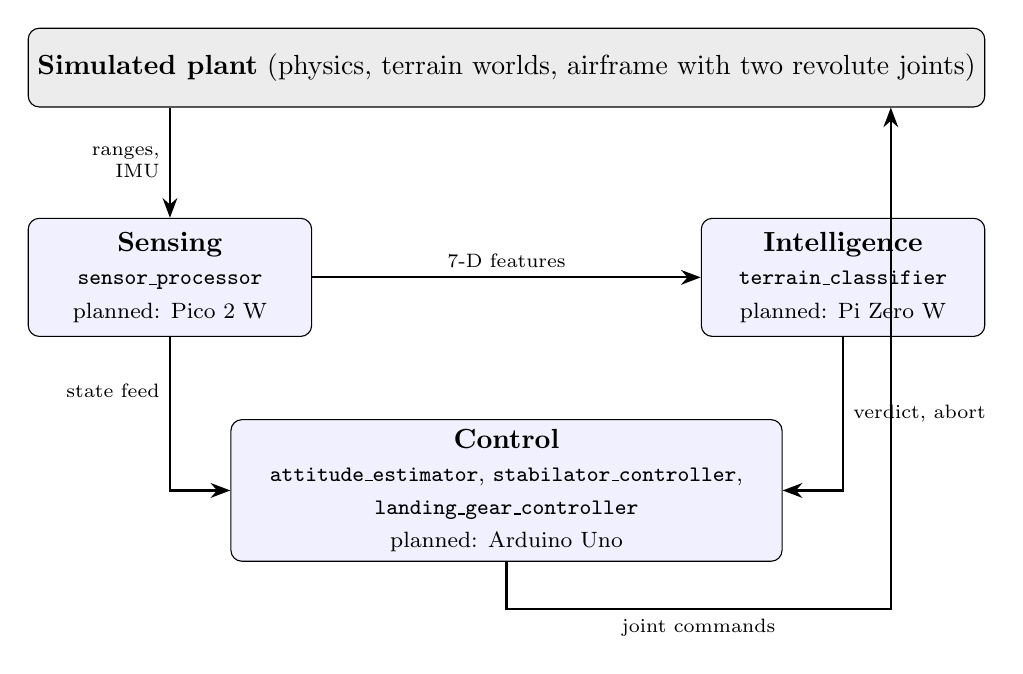
\begin{tikzpicture}[
  box/.style={draw,rounded corners,align=center,minimum width=3.6cm,minimum height=1.5cm,fill=blue!6},
  sim/.style={draw,rounded corners,align=center,minimum width=11.5cm,minimum height=1.0cm,fill=gray!15},
  arr/.style={-{Stealth[length=2.5mm]},thick}
]
\node[sim] (gz) {\textbf{Simulated plant} (physics, terrain worlds, airframe with two revolute joints)};
\node[box,below=14mm of gz.south west,anchor=north west] (sens) {\textbf{Sensing}\\\footnotesize \code{sensor\_processor}\\\footnotesize planned: Pico 2 W};
\node[box,below=14mm of gz.south east,anchor=north east] (int) {\textbf{Intelligence}\\\footnotesize \code{terrain\_classifier}\\\footnotesize planned: Pi Zero W};
\node[box,below=18mm of $(sens)!0.5!(int)$,minimum width=7cm] (ctl) {\textbf{Control}\\\footnotesize \code{attitude\_estimator}, \code{stabilator\_controller},\\\footnotesize \code{landing\_gear\_controller}\\\footnotesize planned: Arduino Uno};
\draw[arr] (gz.south -| sens.north) -- node[left,font=\scriptsize,align=right]{ranges,\\IMU} (sens.north);
\draw[arr] (sens) -- node[above,font=\scriptsize]{7-D features} (int);
\draw[arr] (int.south) -- node[right,font=\scriptsize]{verdict, abort} (int.south |- ctl.east) -- (ctl.east);
\draw[arr] (sens.south) -- node[left,font=\scriptsize,pos=0.35]{state feed} (sens.south |- ctl.west) -- (ctl.west);
\draw[arr] (ctl.south) -- ++(0,-6mm) -| node[pos=0.25,below,font=\scriptsize]{joint commands} ([xshift=-12mm]gz.south east |- gz.south);
\end{tikzpicture}
\caption{Three-domain architecture. Each domain is a set of ROS~2 nodes in the simulation; the boards named are the original deployment plan.}
\label{fig:arch}
\end{figure}
 
\paragraph{Realisations.} The architecture has two realisations in this work. In the simulation, every domain is a set of ROS~2 nodes on a host computer; the boards named in \cref{fig:arch} are the original deployment plan and were not used. In the bench prototype of \cref{sec:bench}, sensing, the readiness decision and the control commands share one Arduino Uno and no classifier is used. There is no hardware-in-the-loop test.
 
\paragraph{Decoupling.} The classifier's output reaches the control domain through a single boolean signal, and the attitude loop is driven by the IMU stream alone. A slow or failed perception node therefore cannot block the stabiliser, although it can leave the abort flag stale.
 
\paragraph{Fail-safe interlock.} When the abort flag is asserted, the gear controller forces the deployment target to the stowed angle irrespective of the request (\cref{sec:gear}).
 
\paragraph{Zero-allocation inference.} The trained classifier is compiled into static C++ comparisons without \code{malloc} or \code{new}, which gives a data-independent bound on the number of operations per decision (\cref{sec:classifier}).
 
%==============================================================
\section{Hardware}\label{sec:hw}
%==============================================================
 
\subsection{Embedded computing targets}
The original design assigns one embedded platform to each domain (\cref{tab:mcu}), following the workload of each: the sensing domain needs bus access and floating-point arithmetic at moderate rates, the intelligence domain only comparisons, and the control domain predictable timing on a simple processor. In this work the simulation runs all domains on a host computer, and the bench prototype uses a single Uno (\cref{sec:bench}).
 
\begin{table}[ht]
\centering
\small
\begin{tabular}{@{}l L{2.7cm} L{4.3cm} L{4.2cm}@{}}
\toprule
\textbf{Domain} & \textbf{Planned platform} & \textbf{Nominal characteristics} & \textbf{Task}\\
\midrule
Sensing & Raspberry Pi Pico 2 W & RP2350 dual-core Arm microcontroller, up to 150\,MHz, 520\,kB SRAM~\cite{rp2350} & Range acquisition and feature extraction\\
Intelligence & Raspberry Pi Zero W & Single-core 1\,GHz ARM11 application processor, 512\,MB RAM & Decision-tree inference, verdict and abort\\
Control & Arduino Uno & ATmega328P 8-bit AVR, 16\,MHz, 2\,kB SRAM~\cite{avr} & Attitude filter, pitch PID, gear actuation\\
\bottomrule
\end{tabular}
\caption{Original embedded plan of the three domains and nominal manufacturer characteristics. None of these boards runs the simulated pipeline.}
\label{tab:mcu}
\end{table}
 
\subsection{Sensors}\label{sec:sensors}
Three sensing modalities are used (\cref{tab:sensors}). Their complementary characteristics are the basis of the perception pipeline.
 
\begin{table}[ht]
\centering
\small
\begin{tabular}{@{}L{2.5cm} L{2.7cm} L{3.4cm} L{5.8cm}@{}}
\toprule
\textbf{Function} & \textbf{Part} & \textbf{Design characteristics} & \textbf{Simulated model}\\
\midrule
Optical ranging ($\times3$) & VL53L0X laser ToF~\cite{vl53} & Narrow beam, $\approx25^\circ$ field of view & $3\times3$ ray fan over $\pm0.04$\,rad, 50\,Hz, range 0.03 to 2.5\,m, 1\,mm resolution, no noise\\
Acoustic ranging & HC-SR04 ultrasonic~\cite{hcsr04} & Wide conical beam, $30^\circ$ to $40^\circ$ & $5\times5$ ray fan over $\pm15^\circ$, 20\,Hz, range 0.02 to 4.0\,m, 1\,cm resolution\\
Attitude & MPU-6500 / MPU-9250 class IMU~\cite{mpu6500,mpu} & Three-axis accelerometer and gyroscope & IMU at the airframe, 100\,Hz; Gaussian noise $\sigma_\omega=10^{-3}$\,rad/s, $\sigma_a=10^{-2}$\,m/s$^2$\\
\bottomrule
\end{tabular}
\caption{Sensors of the system and their simulated models (values from the rig description of the repository).}
\label{tab:sensors}
\end{table}
 
\paragraph{Time-of-flight ranging.} A ToF sensor measures the round-trip time $\Delta t$ of an emitted light pulse and returns $d=c\,\Delta t/2$, with $c$ the speed of light. The narrow beam gives a nearly point-like range measurement with millimetre resolution.
 
\paragraph{Ultrasonic ranging.} The ultrasonic sensor emits a 40\,kHz burst and measures the time until the first significant echo, $d=c_s\,\Delta t/2$, where the speed of sound depends on temperature as $c_s\approx331.3+0.606\,T$\,m/s ($T$ in $^\circ$C). Because the acoustic wavefront is wide, a physical sensor reports the nearest reflecting surface in its footprint. The simulated sonar is a ray fan, and the processing node takes the mean and variance of its valid rays (\cref{sec:texture}).
 
\paragraph{Inertial measurement.} The accelerometer observes the specific force, which for a quasi-static vehicle is the reaction to gravity and therefore encodes pitch and roll; the gyroscope observes angular rate and is accurate in the short term but drifts when integrated.
 
\paragraph{Sensor geometry.} The three ToF sensors form an isosceles triangle on the ventral plate, 0.070\,m below the airframe origin: one fore sensor at $(0.195,\,0)$\,m and a port and a starboard sensor at $(0.125,\,\pm0.039)$\,m, with the sonar at $(0.15,\,0)$\,m (\cref{fig:plate}). The fore sensor is therefore 0.070\,m ahead of the line joining the other two, and the lateral baseline is 0.078\,m; these two baselines are the constants used by the slope computation of \cref{sec:geometry}.
 
\begin{figure}[ht]
\centering
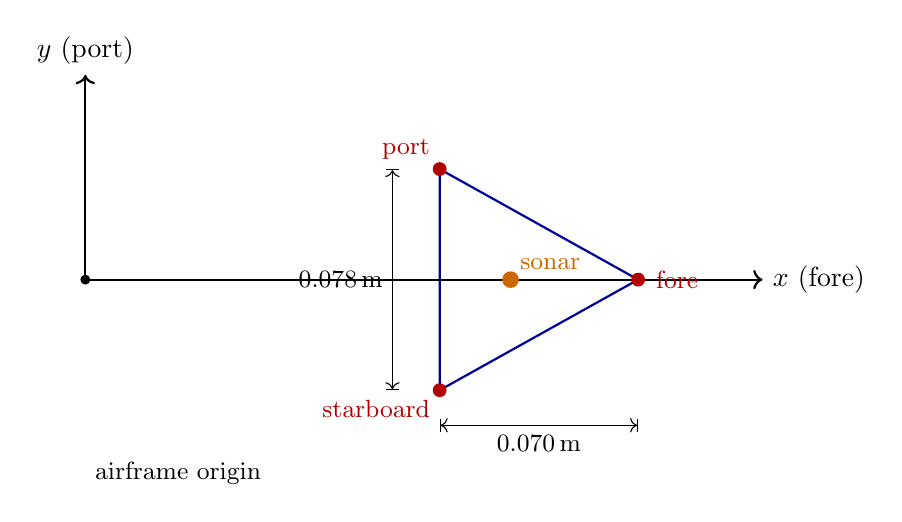
\begin{tikzpicture}[scale=1.0]
  \def\k{36} % cm per m
  \coordinate (F) at ({0.195*\k},0);
  \coordinate (P) at ({0.125*\k},{0.039*\k});
  \coordinate (S) at ({0.125*\k},{-0.039*\k});
  \coordinate (O) at (0,0);
  \draw[thick,blue!60!black] (F) -- (P) -- (S) -- cycle;
  \draw[->,thick] (O) -- (8.6,0) node[right] {$x$ (fore)};
  \draw[->,thick] (O) -- (0,2.6) node[above] {$y$ (port)};
  \fill[red!70!black] (F) circle (2.5pt) node[right=3pt,font=\small] {fore};
  \fill[red!70!black] (P) circle (2.5pt) node[above left,font=\small] {port};
  \fill[red!70!black] (S) circle (2.5pt) node[below left,font=\small] {starboard};
  \fill[orange!80!black] ({0.15*\k},0) circle (3pt) node[above right,font=\small] {sonar};
  \draw[|<->|] ({0.125*\k},-1.85) -- node[below,font=\small] {0.070\,m} ({0.195*\k},-1.85);
  \draw[|<->|] ({0.125*\k-0.6},{-0.039*\k}) -- node[left,font=\small] {0.078\,m} ({0.125*\k-0.6},{0.039*\k});
  \node[font=\small,anchor=north west] at (0,-2.2) {airframe origin};
  \fill (O) circle (1.8pt);
\end{tikzpicture}
\caption{Ventral sensor plate (top view): ToF sensors at $(0.195,0)$, $(0.125,0.039)$ and $(0.125,-0.039)$\,m and sonar at $(0.15,0)$\,m. The fore-aft baseline is 0.070\,m and the lateral baseline 0.078\,m.}
\label{fig:plate}
\end{figure}
 
\subsection{Actuators}
Two actuators are used, both realised as revolute joints (\cref{tab:act}). The physical concept uses SG90 hobby servos~\cite{sg90}. In the simulation each joint is driven by a joint-position controller, which forms the inner loop of a cascade whose outer loop is the attitude or gear command of the control domain.
 
\begin{table}[ht]
\centering
\small
\begin{tabular}{@{}L{2.8cm} L{3.5cm} L{3.6cm} L{4.6cm}@{}}
\toprule
\textbf{Joint} & \textbf{Range} & \textbf{Joint limits} & \textbf{Inner-loop gains}\\
\midrule
Stabilator (T-tail) & $\pm0.4363$\,rad ($\pm25^\circ$) & effort 1.2, speed 6.0\,rad/s & $K_p{=}30$, $K_i{=}0.2$, $K_d{=}1.5$\\
Main landing gear & $0$ to $1.5708$\,rad ($0^\circ$ to $90^\circ$) & effort 2.0, speed 3.5\,rad/s & $K_p{=}25$, $K_i{=}0.2$, $K_d{=}1.0$\\
\bottomrule
\end{tabular}
\caption{Actuated joints of the simulated rig. The inner-loop gains belong to the simulator's joint controllers and are distinct from the outer pitch-stabilisation loop of \cref{sec:pid}.}
\label{tab:act}
\end{table}
 
\subsection{Simulated airframe}
The airframe is modelled as a small fixed-wing aircraft: a cylindrical fuselage of 0.70\,m length and 1.60\,kg mass, a high wing of 0.90\,m span, a T-tail carrying a 0.36\,m horizontal stabilator (0.05\,kg), and a retractable two-wheel main gear (0.11\,kg). The sensor bay is on the ventral side of the fuselage and carries the ToF array and the sonar; the IMU is placed at the centre of gravity. The simulation runs with a 1\,ms physics step. In the three static testbeds the airframe is attached to a fixed test stand 0.70\,m above the ground; in the approach scenario of \cref{sec:supervisor} it is carried along a flight rail. In neither case does the stabilator deflection change the motion of the body. The simulated inertial unit provides accelerations and angular rates only, as does the MPU6500 of the bench prototype.
 
%==============================================================
\section{Algorithms and Methods}\label{sec:algorithms}
%==============================================================
This section develops the algorithms of the three domains. Throughout, $\theta$ denotes pitch, $\phi$ roll, $\vect a=[a_x,a_y,a_z]^\top$ the accelerometer output, $\vect\omega=[\omega_x,\omega_y,\omega_z]^\top$ the gyroscope output and $\Delta t$ the sampling interval.
 
%--------------------------------------------------------------
\subsection{Attitude estimation by complementary filtering}\label{sec:attitude}
%--------------------------------------------------------------
\paragraph{Accelerometer attitude.} For a quasi-static vehicle with a $z$-axis measuring $+g$ when level, the accelerometer reads
\begin{equation}
\vect a=\begin{bmatrix}-g\sin\theta\\ g\cos\theta\sin\phi\\ g\cos\theta\cos\phi\end{bmatrix},
\end{equation}
from which the gravity-referenced angles follow as
\begin{equation}
\theta_{\mathrm{acc}}=\operatorname{atan2}\!\Bigl(-a_x,\ \sqrt{a_y^2+a_z^2}\Bigr),\qquad
\phi_{\mathrm{acc}}=\operatorname{atan2}(a_y,\ a_z).
\label{eq:accangles}
\end{equation}
These estimates are drift-free but corrupted by vehicle acceleration and vibration, because the accelerometer cannot distinguish gravity from linear acceleration.
 
\paragraph{Overflow-safe evaluation.} On an 8-bit AVR target an \code{int} is 16 bits wide. With a $\pm2\,g$ range the raw accelerometer reading is of the order of 16\,384 counts per $g$, and its square ($\approx2.7\times10^8$) overflows a signed 16-bit integer, giving a negative radicand and a \code{NaN} result. The squares in \eqref{eq:accangles} are therefore evaluated after conversion to single-precision floating point.
 
\paragraph{Gyroscope integration.} The angular rates integrate to attitude increments
\begin{equation}
\Delta\theta_{\mathrm{gyro}}=\omega_y\,\Delta t,\qquad \Delta\phi_{\mathrm{gyro}}=\omega_x\,\Delta t,
\end{equation}
which are accurate over short intervals but accumulate sensor bias $b_g$ as a linearly growing error.
 
\paragraph{Fusion.} The two sources have complementary spectra: the gyroscope is reliable at high frequency, the accelerometer at low frequency. The discrete complementary filter blends them with a factor $\alpha\in(0,1)$:
\begin{equation}
\theta_k=\alpha\bigl(\theta_{k-1}+\omega_{y,k}\Delta t\bigr)+(1-\alpha)\,\theta_{\mathrm{acc},k},\qquad
\phi_k=\alpha\bigl(\phi_{k-1}+\omega_{x,k}\Delta t\bigr)+(1-\alpha)\,\phi_{\mathrm{acc},k},
\label{eq:cf}
\end{equation}
with $\alpha=0.90$ and $\Delta t=0.01$\,s (100\,Hz). Yaw is not estimated, because gravity carries no yaw information and the node publishes zero for it.
 
\paragraph{Frequency-domain interpretation.} Taking the $z$-transform of \eqref{eq:cf} for the pitch channel gives
\begin{equation}
\hat\theta(z)=\underbrace{\frac{1-\alpha}{1-\alpha z^{-1}}}_{G_{\mathrm{LP}}(z)}\theta_{\mathrm{acc}}(z)
+\underbrace{\frac{\alpha\,\Delta t}{1-\alpha z^{-1}}}_{}\;\omega_y(z).
\end{equation}
The accelerometer path is a first-order low-pass filter with unit DC gain. If the gyroscope signal is the backward difference of the true angle, $\omega_y=(1-z^{-1})\theta/\Delta t$, its path becomes $\alpha(1-z^{-1})/(1-\alpha z^{-1})$, a high-pass filter, and the two paths sum to
\[
\frac{(1-\alpha)+\alpha(1-z^{-1})}{1-\alpha z^{-1}}=\frac{1-\alpha z^{-1}}{1-\alpha z^{-1}}=1,
\]
so the filter is exactly complementary: it passes the true angle without distortion and only filters the \emph{errors} of the two sensors. The pole at $z=\alpha$ corresponds to a time constant and corner frequency
\begin{equation}
\tau=-\frac{\Delta t}{\ln\alpha}\approx0.095\ \mathrm{s},\qquad f_c=\frac{1}{2\pi\tau}\approx1.7\ \mathrm{Hz}.
\end{equation}
Attitude changes slower than about 1.7\,Hz are therefore taken from the accelerometer, faster ones from the gyroscope.
 
\paragraph{Error analysis.} Two error sources are of interest.
\begin{enumerate}
  \item \emph{Gyroscope bias.} For a constant bias $b_g$ and a constant true angle, the steady state of \eqref{eq:cf} is $\hat\theta-\theta=\alpha\Delta t\,b_g/(1-\alpha)=0.09\,\mathrm{s}\cdot b_g$. A bias of 0.01\,rad/s, for example, produces a bounded error of $9\times10^{-4}$\,rad ($0.05^\circ$) instead of an unbounded drift.
  \item \emph{Accelerometer noise.} For small angles, $\delta\theta_{\mathrm{acc}}\approx\delta a_x/g$, so the simulated noise $\sigma_a=0.01$\,m/s$^2$ gives $\approx1.0\times10^{-3}$\,rad per sample. The low-pass path reduces the standard deviation by $\sqrt{(1-\alpha)/(1+\alpha)}\approx0.23$, leaving $\approx2.3\times10^{-4}$\,rad ($0.013^\circ$).
\end{enumerate}
 
\begin{algorithm}[ht]
\caption{Complementary filter update (executed at 100\,Hz)}\label{alg:cf}
\begin{algorithmic}[1]
\Require raw $a_x,a_y,a_z$, $\omega_x,\omega_y,\omega_z$, previous state $(\theta_{k-1},\phi_{k-1})$, $\alpha$, $\Delta t$
\Ensure filtered pitch $\theta_k$ and roll $\phi_k$
\State convert $a_x,a_y,a_z$ to single-precision floating point
\State $\theta_{\mathrm{acc}}\gets\operatorname{atan2}(-a_x,\sqrt{a_y^2+a_z^2})$
\State $\phi_{\mathrm{acc}}\gets\operatorname{atan2}(a_y,a_z)$
\State $\theta_k\gets\alpha(\theta_{k-1}+\omega_y\Delta t)+(1-\alpha)\theta_{\mathrm{acc}}$
\State $\phi_k\gets\alpha(\phi_{k-1}+\omega_x\Delta t)+(1-\alpha)\phi_{\mathrm{acc}}$
\State publish $(\phi_k,\theta_k)$ as the attitude estimate
\end{algorithmic}
\end{algorithm}
 
%--------------------------------------------------------------
\subsection{Active pitch stabilisation}\label{sec:pid}
%--------------------------------------------------------------
\paragraph{Purpose.} Terrain geometry is measured in the sensor frame; if the fuselage pitches during descent, the three ToF beams no longer point along the local vertical and the apparent slope is biased. The horizontal stabilator is therefore driven by a closed-loop controller that regulates the estimated pitch to a setpoint $\theta_{\mathrm{ref}}$ (default $0$\,rad). Deflecting the tail surface changes the tail lift and hence the pitching moment about the centre of gravity, which is the actuation path exploited by the controller. In the simulation this path is not closed physically, because the airframe is held by a test stand or a flight rail; the loop acts on the estimated pitch and drives the stabilator joint.
 
\paragraph{Control law.} With the error $e_\theta(t)=\theta_{\mathrm{ref}}-\hat\theta(t)$ the continuous PID law is
\begin{equation}
u(t)=K_p\,e_\theta(t)+K_i\!\int_0^t e_\theta(\tau)\,d\tau+K_d\,\frac{de_\theta(t)}{dt}.
\end{equation}
The proportional term provides the primary restoring action, the integral term removes steady-state error caused by constant disturbances such as trim offsets, and the derivative term adds damping and limits overshoot.
 
\paragraph{Discrete implementation and anti-windup.} At 100\,Hz the loop is realised as
\begin{align}
S_k&=\operatorname{clamp}\bigl(S_{k-1}+e_k\,\Delta t,\ -S_{\max},\ S_{\max}\bigr),\\
D_k&=K_d\,\frac{e_k-e_{k-1}}{\Delta t},\\
u_k&=\operatorname{sat}\bigl(K_p\,e_k+K_i\,S_k+D_k,\ -u_{\max},\ u_{\max}\bigr),\qquad u_{\max}=0.4363\ \mathrm{rad},
\end{align}
The command is saturated at the mechanical limit of the stabilator. Without further measures, an integrator would continue to accumulate while the actuator is saturated (for example during a strong gust) and cause a large overshoot when the error finally changes sign. Clamping the integral state $S_k=\int e\,dt$ to $[-S_{\max},S_{\max}]$ prevents this \emph{integrator windup}~\cite{astrom}. The loop is executed for every attitude sample, with the derivative taken on the error and a fall-back step of 10\,ms if the measured step is non-positive or longer than 0.2\,s. The gains are $K_p=1.8$, $K_i=0.05$ and $K_d=0.25$, with $S_{\max}=0.20$\,rad\,s; they are run-time parameters of the node. The resulting command is sent to the simulated stabilator joint, whose own position controller (\cref{tab:act}) acts as the fast inner loop of the cascade.
 
\begin{algorithm}[ht]
\caption{Discrete PID pitch stabiliser with anti-windup (100\,Hz)}\label{alg:pid}
\begin{algorithmic}[1]
\Require estimated pitch $\hat\theta$, setpoint $\theta_{\mathrm{ref}}$, gains $K_p,K_i,K_d$, limits $S_{\max},u_{\max}$, state $(S_{k-1},e_{k-1})$
\Ensure stabilator command $u_k$
\State $e_k\gets\theta_{\mathrm{ref}}-\hat\theta$
\State $S_k\gets\operatorname{clamp}(S_{k-1}+e_k\Delta t,\,-S_{\max},\,S_{\max})$
\State $D_k\gets K_d\,(e_k-e_{k-1})/\Delta t$
\State $u_k\gets\operatorname{clamp}(K_p e_k+K_i S_k+D_k,\,-u_{\max},\,u_{\max})$
\State store $(S_k,e_k)$ and publish $u_k$ to the stabilator
\end{algorithmic}
\end{algorithm}
 
 
%--------------------------------------------------------------
\subsection{Terrain slope from the ToF triangle}\label{sec:geometry}
%--------------------------------------------------------------
\paragraph{Range extraction.} Each ToF sensor delivers a scan of nine rays. The processing node keeps, for every sensor, the minimum range among the rays that are finite and inside the sensor limits, and holds the most recent value; if a scan contains no valid ray, the value 0.85\,m is used. Denote the three values $d_f$ (fore), $d_p$ (port) and $d_s$ (starboard). There is no averaging window and no freshness check: the features are computed from the latest retained scans.
 
\paragraph{Planar model.} With the sensor plate level and the beams vertical, a locally planar surface with gradients $g_x$ (along the fore axis) and $g_y$ (along the port axis) produces ranges
\begin{equation}
d_i=d_0-\bigl(g_x\,x_i+g_y\,y_i\bigr),\qquad i\in\{f,p,s\},
\label{eq:plane}
\end{equation}
where $d_0$ is the range at the origin of the plate and $(x_i,y_i)$ are the sensor positions of \cref{fig:plate}. Two differences isolate the gradients. The fore sensor and the midpoint of the other two are separated by $\Delta x=0.070$\,m along $x$ and have the same $y$, and the port and starboard sensors are separated by $\Delta y=0.078$\,m along $y$ at the same $x$. Hence
\begin{equation}
d_f-\tfrac12(d_p+d_s)=-g_x\,\Delta x,\qquad d_p-d_s=-g_y\,\Delta y .
\end{equation}
 
\paragraph{Implemented estimate.} The sensing node converts the two differences into angles,
\begin{equation}
\beta_x=\operatorname{atan2}\!\bigl(d_f-\tfrac12(d_p+d_s),\ 0.070\bigr),\qquad
\beta_y=\operatorname{atan2}\!\bigl(d_p-d_s,\ 0.078\bigr),\qquad
\beta=\sqrt{\beta_x^{2}+\beta_y^{2}} .
\label{eq:slope}
\end{equation}
For a plane inclined along one axis only, $|\beta_x|=\arctan|g_x|$ is the exact inclination of the surface, because the range difference divided by the baseline equals the rise over the run. For a plane inclined along both axes, $\beta$ approximates the true inclination $\arctan\sqrt{g_x^2+g_y^2}$ by a root-sum-square of the per-axis angles; for $g_x=g_y=0.2$ the two values are $0.279$ and $0.276$\,rad. The sign of $\beta_x$ and $\beta_y$ depends on whether the ground rises or falls along the axis, and only the magnitude $\beta\ge0$ (and $|\beta_y|$) is used downstream. The computation uses the two baseline constants directly rather than a surface normal from the cross product of the span vectors, and it does not use the IMU.
 
\paragraph{Consequences of the assumptions.} The estimate is valid only if the plate is level. If the aircraft is pitched by $\theta$, the beams are no longer vertical and $\beta_x$ is shifted by roughly $\theta$; since the runtime does not subtract the filtered attitude, body pitch appears as terrain slope. This is the reason for stabilising pitch (\cref{sec:pid}), but in the simulation the airframe is held by a stand or a rail, so the coupling is never exercised. The estimate also treats the 0.070\,m by 0.078\,m patch as planar, so it measures the surface at a scale of about 0.1\,m and cannot see slopes of larger extent or smaller obstacles.
 
\paragraph{Noise sensitivity.} The short baselines amplify range noise. For independent range errors of standard deviation $\sigma$, $\operatorname{Var}\bigl(d_f-\tfrac12(d_p+d_s)\bigr)=\tfrac32\sigma^2$ and $\operatorname{Var}(d_p-d_s)=2\sigma^2$, so for small angles
\begin{equation}
\sigma_{\beta_x}\approx\frac{\sqrt{1.5}\,\sigma}{0.070}\approx17.5\,\sigma\ \mathrm{rad/m},\qquad
\sigma_{\beta_y}\approx\frac{\sqrt2\,\sigma}{0.078}\approx18.1\,\sigma\ \mathrm{rad/m}.
\end{equation}
A range noise of 2\,mm, which is of the order expected for a real ToF module, would give about 0.035\,rad ($2^\circ$) per axis. The simulated ToF sensors are noise-free with 1\,mm resolution, so this noise is not present in the simulation results.
 
%--------------------------------------------------------------
\subsection{Optical-acoustic comparison}\label{sec:texture}
%--------------------------------------------------------------
The ToF beams are narrow and the acoustic fan is wide, so the two sensor types sample the surface at different scales. The sensing node computes two quantities that compare them.
 
\paragraph{Mean difference.} The optical altitude is the mean of the three ToF ranges, $\bar d_{\mathrm{ToF}}=\tfrac13(d_f+d_p+d_s)$, and the acoustic range $\bar d_{\mathrm{sonar}}$ is the mean of the valid rays of the latest sonar scan. Their difference is
\begin{equation}
\Delta d=\bar d_{\mathrm{sonar}}-\bar d_{\mathrm{ToF}} .
\end{equation}
The oblique rays of the $\pm15^\circ$ fan travel farther than a vertical ray, which gives $\Delta d$ a positive offset on flat ground, and surface relief inside the acoustic footprint changes it further. In the three static worlds $\Delta d$ lies between 0.010 and 0.033\,m (\cref{tab:featvals}). The original concept used this difference as a cue for penetrable vegetation, where the optical and acoustic channels may see different surfaces. The simulated canopy is a solid body, no optical penetration is modelled, the sign of $\Delta d$ in the synthetic canopy is not consistently positive, and no real-material experiment was made. The cue is therefore computed but is not validated as a vegetation detector.
 
\paragraph{Scan variance.} The second quantity is the population variance of the valid sonar rays within one scan,
\begin{equation}
\sigma^2_{\mathrm{sonar}}=\frac1n\sum_{j=1}^{n}\bigl(r_j-\bar d_{\mathrm{sonar}}\bigr)^2,\qquad \sigma^2_{\mathrm{sonar}}\ge10^{-5}\ \mathrm{m^2},
\end{equation}
which measures the relief of the surface across the acoustic cone at a single instant. It is not a temporal variance.
 
%--------------------------------------------------------------
\subsection{Feature extraction}\label{sec:features}
%--------------------------------------------------------------
\paragraph{Spatial variance of the ToF ranges.} The roughness measure is the population variance of the three ToF ranges,
\begin{equation}
\sigma^2_{\mathrm{sp}}=\frac13\sum_{i\in\{f,p,s\}}\bigl(d_i-\bar d_{\mathrm{ToF}}\bigr)^2,\qquad\sigma^2_{\mathrm{sp}}\ge10^{-5}\ \mathrm{m^2}.
\label{eq:spvar}
\end{equation}
For a plane \eqref{eq:plane} the range deviations are $-g_x(x_i-\bar x)-g_y(y_i-\bar y)$. With the plate geometry of \cref{fig:plate}, the variance of the $x$ coordinates is $\tfrac13\sum(x_i-\bar x)^2=1.089\times10^{-3}$\,m$^2$ and that of the $y$ coordinates is $1.014\times10^{-3}$\,m$^2$, and the cross term vanishes because the sensors are symmetric about $y=0$. Therefore
\begin{equation}
\sigma^2_{\mathrm{sp}}=1.089\times10^{-3}\,g_x^2+1.014\times10^{-3}\,g_y^2\ \ \mathrm{m^2}.
\label{eq:spmodel}
\end{equation}
On a planar patch the roughness measure is thus a function of the same gradients as the slope, and it departs from this relation only when the ranges are not coplanar, which is the case it is meant to detect. For the Beta ramp the apparent slope of $0.348$\,rad gives $g_x=\tan0.348=0.363$ and a predicted variance of $1.4\times10^{-4}$\,m$^2$, in agreement with the measured $1.43\times10^{-4}$\,m$^2$ (\cref{tab:featvals}).
 
\paragraph{Feature vector.} The node publishes the vector of \cref{tab:features} on a 20\,ms timer (nominal 50\,Hz) and the altitude $\bar d_{\mathrm{ToF}}$ on a separate topic. The column names of the recorded dataset (\cref{sec:classifier}) predate the current code, and their meaning differs for three entries: the fourth feature is a variance within one sonar scan rather than a temporal variance of $\Delta d$, the sixth is the magnitude of the roll slope and not the gyroscope norm, and the seventh repeats the total slope and is not a filtered attitude error. \Cref{tab:features} lists what the runtime computes.
 
\begin{table}[ht]
\centering
\small
\begin{tabular}{@{}c L{3.4cm} L{5.9cm} l c@{}}
\toprule
\textbf{Index} & \textbf{Quantity} & \textbf{Definition} & \textbf{Unit} & \textbf{Used}\\
\midrule
0 & Mean ToF range & $\bar d_{\mathrm{ToF}}$ & m & no\\
1 & Spatial variance & $\sigma^2_{\mathrm{sp}}$, \eqref{eq:spvar} & m$^2$ & yes\\
2 & Optical-acoustic difference & $\Delta d=\bar d_{\mathrm{sonar}}-\bar d_{\mathrm{ToF}}$ & m & no\\
3 & Sonar scan variance & $\sigma^2_{\mathrm{sonar}}$ & m$^2$ & no\\
4 & Total slope & $\beta$, \eqref{eq:slope} & rad & no\\
5 & Roll slope magnitude & $|\beta_y|$ & rad & no\\
6 & Total slope (repeated) & $\beta$, \eqref{eq:slope} & rad & yes\\
\bottomrule
\end{tabular}
\caption{Feature vector computed by the sensing node. The last column states whether the trained tree reads the entry.}
\label{tab:features}
\end{table}
 
\begin{algorithm}[ht]
\caption{Feature extraction cycle of the sensing node (every 20\,ms)}\label{alg:features}
\begin{algorithmic}[1]
\Require latest ToF scans $(d_f,d_p,d_s)$ (minimum valid ray, fallback 0.85\,m), latest sonar statistics $(\bar d_{\mathrm{sonar}},\sigma^2_{\mathrm{sonar}})$
\Ensure feature vector $\vect x\in\mathbb R^7$ and altitude $\bar d_{\mathrm{ToF}}$
\State $\bar d_{\mathrm{ToF}}\gets(d_f+d_p+d_s)/3$
\State $\sigma^2_{\mathrm{sp}}\gets\max\bigl(10^{-5},\ \tfrac13\sum_i(d_i-\bar d_{\mathrm{ToF}})^2\bigr)$
\State $\Delta d\gets\bar d_{\mathrm{sonar}}-\bar d_{\mathrm{ToF}}$
\State $\beta_x\gets\operatorname{atan2}(d_f-\tfrac12(d_p+d_s),\,0.070)$;\quad $\beta_y\gets\operatorname{atan2}(d_p-d_s,\,0.078)$
\State $\beta\gets\sqrt{\beta_x^2+\beta_y^2}$
\State $\vect x\gets[\bar d_{\mathrm{ToF}},\ \sigma^2_{\mathrm{sp}},\ \Delta d,\ \sigma^2_{\mathrm{sonar}},\ \beta,\ |\beta_y|,\ \beta]$
\State publish $\vect x$ and $\bar d_{\mathrm{ToF}}$
\end{algorithmic}
\end{algorithm}
 
%--------------------------------------------------------------
\subsection{Edge-AI terrain classifier}\label{sec:classifier}
%--------------------------------------------------------------
\paragraph{Task and labels.} The classifier maps the feature vector $\vect x\in\mathbb R^7$ to a class $y\in\{0,1,2\}$. The labels describe the suitability of the terrain below the aircraft for landing (\cref{tab:labels}). Class 0 (\textsc{safe}) denotes a level, rigid surface on which the gear may be deployed. The two unsafe classes distinguish the \emph{reason} for rejecting the terrain: class 1 (\textsc{unsafe\_slope}) denotes a geometric hazard, an inclined surface that risks rollover, whereas class 2 (\textsc{unsafe\_vegetation}) denotes an irregular surface of mounds and a canopy body, where the footing is uncertain. Both unsafe classes have the same operational consequence: the abort flag is asserted for every verdict other than \textsc{safe}, which inhibits gear deployment (\cref{sec:gear}).
 
\begin{table}[ht]
\centering
\small
\begin{tabular}{@{}L{2.9cm} L{1.7cm} L{5.6cm} L{4.5cm}@{}}
\toprule
\textbf{Label} & \textbf{Testbed} & \textbf{Terrain} & \textbf{Intended signature}\\
\midrule
0 \textsc{safe} & Alpha & Flat ground plane & Near-zero slope and roughness\\
1 \textsc{unsafe\_slope} & Beta & $20^\circ$ inclined ramp and a stepped curb block & Large slope, small roughness on the planar ramp\\
2 \textsc{unsafe\_vegetation} & Gamma & Three box-shaped mounds (0.08 to 0.14\,m high) and a central solid cylinder (0.18\,m radius, 0.16\,m high) & Large slope and roughness within the sensor patch\\
\bottomrule
\end{tabular}
\caption{Class labels, the testbed that produces each class and the intended signature.}
\label{tab:labels}
\end{table}
 
\paragraph{Dataset.} A recording node subscribes to the feature topic, keeps the first seven values of each message together with the label of the selected world, and writes one row per message to a comma-separated file; 500 samples per world is the default, so one run in each testbed gives 1\,500 labelled vectors (500 per class). Two properties of the data matter for the interpretation of the results. First, the labels are properties of the \emph{world}: every row inherits the label of its testbed irrespective of the instantaneous sensor reading. Second, the rig is static, the sensors are noise-free and the geometry is fixed, so the recorded vectors of one world are almost identical (\cref{tab:dataset}). Most columns have zero standard deviation within a class: only the angular-rate column and the last column vary, with standard deviations of about $6\times10^{-4}$ and $2\times10^{-4}$, respectively. The dataset therefore consists of three tight clusters rather than three distributions of terrain.
 
\begin{table}[ht]
\centering
\small
\begin{tabular}{@{}l r r r@{}}
\toprule
\textbf{Column (recorded name)} & \textbf{Class 0} & \textbf{Class 1} & \textbf{Class 2}\\
\midrule
\code{mean\_tof} (m) & 1.640000 & 1.440778 & 1.506667\\
\code{spatial\_variance} (m$^2$) & 0 & 0.000144 & 0.001422\\
\code{delta\_d} (m) & 0.057811 & 0.051345 & 0.191144\\
\code{delta\_d\_variance} & 0 & 0 & 0\\
\code{beta\_slope} (rad) & 0 & 0.275867 & 0.726643\\
\code{omega\_norm} (rad/s) & 0.001647 & 0.001597 & 0.001550\\
\code{tilt\_error} (rad), mean & 0.000238 & 0.275854 & 0.726638\\
\code{tilt\_error}, minimum & 0.000000 & 0.274958 & 0.726070\\
\code{tilt\_error}, maximum & 0.000753 & 0.276555 & 0.727235\\
\bottomrule
\end{tabular}
\caption{Class means of the recorded dataset (500 samples per class). The standard deviation within a class is zero for every row except \code{omega\_norm} (about $6\times10^{-4}$) and \code{tilt\_error} (about $2\times10^{-4}$).}
\label{tab:dataset}
\end{table}

\noindent
The dataset was recorded with an earlier version of the sensing node. Its values differ from the live runtime values of \cref{tab:featvals} (for example the mean range of Beta is 1.44\,m in the dataset and 0.53\,m in the verification run, and the slope 0.276 against 0.348\,rad), and the repository advises recording the actual feature definitions alongside any new dataset. The tree was not retrained for the current runtime; its thresholds are applied to the live features, as discussed below.
 
\paragraph{Model choice.} A classification tree (CART~\cite{cart}) was selected. An initial concept considered a small multilayer perceptron with quantisation for microcontrollers. A tree offers several advantages for this application: (i) its decision path is a short sequence of threshold comparisons that can be inspected and audited, which matters for a safety function; (ii) it needs no matrix arithmetic or activation functions; (iii) it compiles into code with a constant bound on the operations and no dynamic allocation; and (iv) the features are physically meaningful, so that axis-aligned splits are natural.
 
\paragraph{Induction.} A tree is grown greedily. For a node holding the sample set $S$ with class proportions $p_k$, the Gini impurity is
\begin{equation}
G(S)=1-\sum_{k=0}^{2}p_k^2 ,
\end{equation}
which is $0$ for a pure node and $2/3$ for three equally frequent classes. For every feature $j$ and candidate threshold $t$ (the midpoints between consecutive sorted feature values) the set is split into $S_L=\{\vect x:x_j\le t\}$ and $S_R=S\setminus S_L$, and the split with the largest impurity decrease is chosen,
\begin{equation}
(j^\ast,t^\ast)=\arg\max_{j,t}\ \Bigl[G(S)-\tfrac{|S_L|}{|S|}G(S_L)-\tfrac{|S_R|}{|S|}G(S_R)\Bigr].
\label{eq:gini}
\end{equation}
The procedure recurses on $S_L$ and $S_R$ until a node is pure or the maximum depth is reached; a leaf predicts the majority class of its samples (\cref{alg:cart}). A depth limit of four bounds the model to at most 16 leaves and 15 decision nodes and caps inference at four comparisons per decision.
 
\begin{algorithm}[ht]
\caption{Greedy induction of a depth-limited classification tree}\label{alg:cart}
\begin{algorithmic}[1]
\Require labelled set $S$, current depth $\ell$, maximum depth $\ell_{\max}=4$
\Ensure tree node
\Function{Grow}{$S,\ell$}
  \If{$G(S)=0$ \textbf{or} $\ell=\ell_{\max}$} \State \Return Leaf(majority class of $S$) \EndIf
  \State $(j^\ast,t^\ast)\gets\arg\max_{j,t}$ impurity decrease of \eqref{eq:gini}
  \State $S_L\gets\{\vect x\in S: x_{j^\ast}\le t^\ast\}$;\quad $S_R\gets S\setminus S_L$
  \State \Return Node($j^\ast,t^\ast$, \Call{Grow}{$S_L,\ell+1$}, \Call{Grow}{$S_R,\ell+1$})
\EndFunction
\end{algorithmic}
\end{algorithm}
 
\paragraph{Training configuration.} The parameters of the training procedure are listed in \cref{tab:trainconf}. The dataset is split 75\,\%/25\,\% into 1\,125 training and 375 test samples with stratification, and a fixed random seed makes the split and the tree reproducible. Training uses the scikit-learn implementation~\cite{sklearn}; every parameter not listed takes the library default.
 
\begin{table}[ht]
\centering
\small
\begin{tabular}{@{}L{4.6cm} L{10.2cm}@{}}
\toprule
\textbf{Parameter} & \textbf{Value}\\
\midrule
Algorithm & CART classification tree (\code{DecisionTreeClassifier})\\
Inputs & 7 features (\cref{tab:features}), single precision at inference\\
Classes & 3 (\textsc{safe}, \textsc{unsafe\_slope}, \textsc{unsafe\_vegetation})\\
Samples & 1\,500 (1\,125 training, 375 test)\\
Train/test split & 75\,\%/25\,\%, stratified by class, random seed 42\\
Split criterion & Gini impurity, \eqref{eq:gini}\\
Maximum depth & 4\\
Random seed of the tree & 42\\
Other parameters & Library defaults: all seven features considered at every split, minimum 2 samples to split a node, minimum 1 sample per leaf, no class weights, no pruning\\
\bottomrule
\end{tabular}
\caption{Training configuration of the terrain classifier.}
\label{tab:trainconf}
\end{table}
 
\paragraph{Learned model.} Although the depth limit is four, the fitted tree is small (\cref{fig:tree}): two decision nodes and three leaves, using two of the seven feature slots (indices 6 and 1). Growth stopped after two levels because every leaf was pure.
\begin{enumerate}
  \item \emph{Root split on feature 6.} Samples with a value of at most $0.137855$\,rad ($\approx7.9^\circ$) are classified \textsc{safe}. In the dataset, the largest class-0 value is $0.000753$ and the smallest class-1 value is $0.274958$, and $(0.000753+0.274958)/2=0.137855$, so the threshold is the midpoint of the gap between the flat-ground cluster and the ramp cluster. It is a property of the data gap and not a certified slope limit. In the current runtime, feature 6 is the total slope $\beta$ of \eqref{eq:slope}, so the node acts as a slope detector.
  \item \emph{Second split on the spatial variance.} Among the remaining samples, those with $\sigma^2_{\mathrm{sp}}\le0.000783$\,m$^2$ are classified \textsc{unsafe\_slope} and the others \textsc{unsafe\_vegetation}. Again $(0.000144+0.001422)/2=0.000783$, the midpoint between the Beta and Gamma clusters. For planar returns inclined along the fore axis, \eqref{eq:spmodel} places this threshold at $g_x=\sqrt{0.000783/0.001089}=0.85$, an inclination of about $40^\circ$. On such surfaces the second split is thus equivalent to a second slope threshold, and it separates the \textsc{unsafe\_vegetation} class from the \textsc{unsafe\_slope} class by the magnitude of the height differences within the 0.1\,m patch.
\end{enumerate}
 
\begin{figure}[ht]
\centering
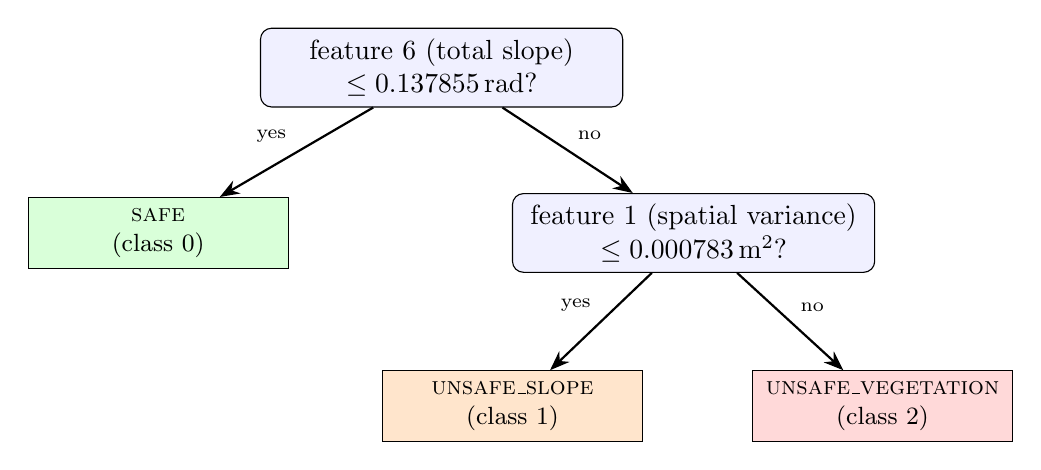
\begin{tikzpicture}[
  dec/.style={draw,rounded corners,align=center,fill=blue!6,minimum width=4.6cm,minimum height=1.0cm},
  leaf/.style={draw,align=center,minimum width=3.3cm,minimum height=0.9cm,font=\small},
  arr/.style={-{Stealth[length=2.5mm]},thick}
]
\node[dec] (n1) at (0,0) {feature 6 (total slope)\\$\le0.137855$\,rad?};
\node[leaf,fill=green!15] (l0) at (-3.6,-2.1) {\textsc{safe}\\(class 0)};
\node[dec] (n2) at (3.2,-2.1) {feature 1 (spatial variance)\\$\le0.000783$\,m$^2$?};
\node[leaf,fill=orange!20] (l1) at (0.9,-4.3) {\textsc{unsafe\_slope}\\(class 1)};
\node[leaf,fill=red!15] (l2) at (5.6,-4.3) {\textsc{unsafe\_vegetation}\\(class 2)};
\draw[arr] (n1) -- node[above left,font=\scriptsize]{yes} (l0);
\draw[arr] (n1) -- node[above right,font=\scriptsize]{no} (n2);
\draw[arr] (n2) -- node[above left,font=\scriptsize]{yes} (l1);
\draw[arr] (n2) -- node[above right,font=\scriptsize]{no} (l2);
\end{tikzpicture}
\caption{Trained classification tree: two decision nodes and three leaves, using two of the seven features.}
\label{fig:tree}
\end{figure}
\noindent 
The optical-acoustic features of \cref{sec:texture} (indices 2 and 3) were not selected, because the two thresholds above already separate the clusters perfectly. These data therefore give no evidence that the optical-acoustic cue adds information.
 
\paragraph{Compilation to C++.} After training, the tree is traversed recursively and each internal node is emitted as an \code{if}/\code{else} comparison of a feature against a single-precision threshold, each leaf as a \code{return} of the class index (\cref{alg:codegen}). The generated header contains a single function, \code{predict\_terrain(const float*)}, whose structure is
\begin{lstlisting}
inline int32_t predict_terrain(const float * features)
{
  if (features[j] <= t) {      // internal node
    ...                        // left subtree
  } else {
    ...                        // right subtree
  }                            // leaf: return <class index>;
}
\end{lstlisting}
It depends only on \code{<cstdint>}, performs no dynamic allocation and has a data-independent upper bound of four comparisons; the trained tree needs two. The thresholds are emitted with six decimal places in single precision.
 
\begin{algorithm}[ht]
\caption{Generation of the inference code from a trained tree}\label{alg:codegen}
\begin{algorithmic}[1]
\Require trained tree, feature names
\Ensure C++ source of \code{predict\_terrain}
\Function{Emit}{node, depth}
  \If{node is internal}
    \State write ``\code{if (features[j] <= t) \{}''
    \State \Call{Emit}{left child, depth+1}
    \State write ``\code{\} else \{}''
    \State \Call{Emit}{right child, depth+1}
    \State write ``\code{\}}''
  \Else
    \State write ``\code{return} $\arg\max_k$ (class counts of node)''
  \EndIf
\EndFunction
\end{algorithmic}
\end{algorithm}
 
\paragraph{Runtime behaviour.} The classifier node evaluates every incoming feature vector and publishes the verdict and the abort flag once per accepted message, with the abort flag set for every verdict other than \textsc{safe}. Messages with fewer than seven elements are rejected. The verdict is not filtered: there is no debouncing or hysteresis, so the abort flag follows the instantaneous classification.
 
\paragraph{Safety-oriented metrics.} Because the error costs are asymmetric, overall accuracy is not the decisive figure. Two dedicated metrics are used,
\begin{equation}
\mathrm{FSR}=\frac{|\{i:y_i\neq0\wedge\hat y_i=0\}|}{|\{i:y_i\neq0\}|},\qquad
R_{\mathrm{safe}}=\frac{|\{i:y_i=0\wedge\hat y_i=0\}|}{|\{i:y_i=0\}|},
\end{equation}
the false-safe rate (FSR) and the recall of the safe class, with targets $\mathrm{FSR}=0$ and $R_{\mathrm{safe}}\ge0.98$. The Gini criterion treats all misclassifications equally, so the safety requirement is enforced by evaluation rather than by the training objective.
 
\paragraph{Test-set results.} The tree was evaluated on the 375 held-out samples, which contain 125 samples of each class. The confusion matrix is shown in \cref{tab:confusion} and \cref{fig:confusion}: all 375 samples were classified correctly, so accuracy, precision, recall and F1-score are all $1.00$, $\mathrm{FSR}=0/250=0$ and $R_{\mathrm{safe}}=125/125=1$.
 
\begin{table}[ht]
\centering
\small
\begin{tabular}{@{}l c c c@{}}
\toprule
\textbf{Actual $\backslash$ predicted} & \textsc{safe} & \textsc{unsafe\_slope} & \textsc{unsafe\_vegetation}\\
\midrule
\textsc{safe} & 125 & 0 & 0\\
\textsc{unsafe\_slope} & 0 & 125 & 0\\
\textsc{unsafe\_vegetation} & 0 & 0 & 125\\
\bottomrule
\end{tabular}
\caption{Confusion matrix on the 375-sample test set.}
\label{tab:confusion}
\end{table}
 
\begin{figure}[ht]
\centering
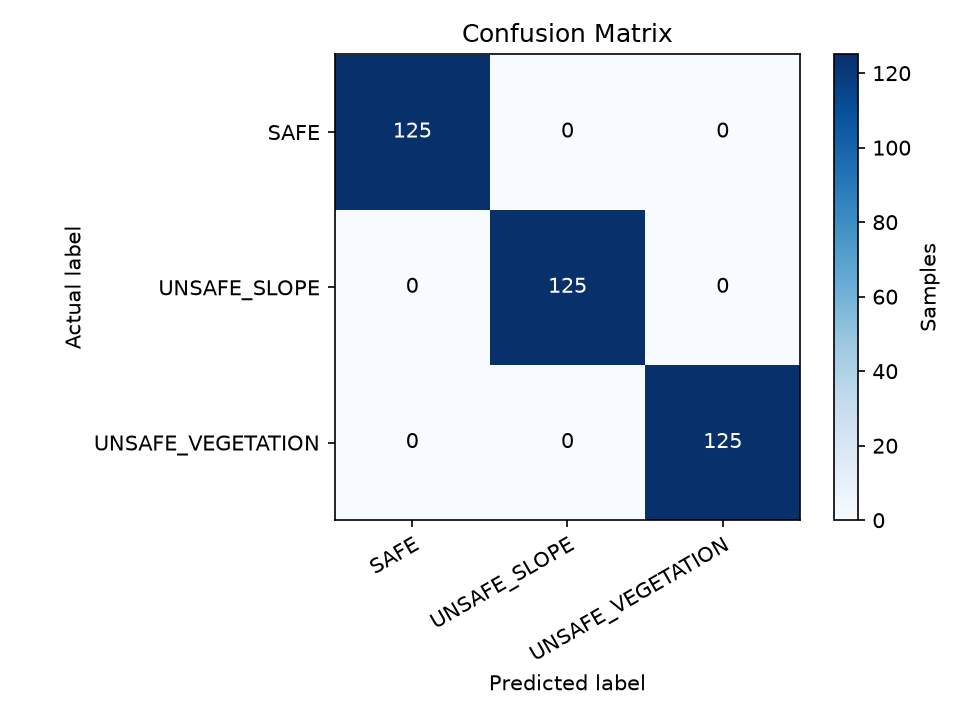
\includegraphics[width=0.68\linewidth]{figs/confusion_matrix.png}
\caption{Confusion matrix of the classifier on the held-out test set.}
\label{fig:confusion}
\end{figure}
 
This result must be read with the data in mind. Because the classes are separated by gaps of $0.27$\,rad and $0.0013$\,m$^2$, much larger than the spread within a class, and the thresholds are the midpoints of those gaps, any random split yields a perfect score. The test samples are in addition drawn from the same runs as the training samples and carry per-world labels. The score therefore shows that the three synthetic terrain types are separable, and it does not estimate performance on unseen terrain.
 
\paragraph{Execution time.} Since a decision requires at most four comparisons (two in the trained tree), the latency is dominated by memory access and is of the order of tens of nanoseconds on the host (\cref{sec:validation}).
 
%--------------------------------------------------------------
\subsection{Gear control and safety interlock}\label{sec:gear}
%--------------------------------------------------------------
\paragraph{Interlocked target.} Let $D_k\in\{0,1\}$ be the deploy request, published by the supervisor or by an operator, and $A_k\in\{0,1\}$ the abort flag. The target gear angle is
\begin{equation}
q^\ast_k=\frac{\pi}{2}\,D_k\,(1-A_k)
\end{equation}
so that $q^\ast_k=0$ (stowed) whenever $A_k=1$, regardless of the request. The interlock thus has priority over the command. The controller contains no altitude logic of its own; the decision to request deployment belongs to the supervisor (\cref{sec:supervisor}) or the operator.
 
\paragraph{Rate limiting.} To avoid abrupt mechanical loading and to bound the actuation speed, the target is passed through a rate limiter,
\begin{equation}
q_k=q_{k-1}+\operatorname{clamp}\bigl(q^\ast_k-q_{k-1},\ -\dot q_{\max}\Delta t,\ \dot q_{\max}\Delta t\bigr),
\end{equation}
with $\dot q_{\max}=0.50$\,rad/s and $\Delta t=0.02$\,s (50\,Hz), i.e.\ a maximum step of 0.01\,rad. A full sweep takes $(\pi/2)/\dot q_{\max}\approx3.14$\,s. Because the same limiter acts when the abort asserts during deployment, the gear reverses at the permitted speed and reaches the stowed angle in at most 3.14\,s. The published gear status is the controller's own trajectory $q_k$ and not a measurement of the joint position.
 
\begin{algorithm}[ht]
\caption{Landing gear controller step with abort interlock (50\,Hz)}\label{alg:gear}
\begin{algorithmic}[1]
\Require deploy request $D$, abort flag $A$, current command $q_{k-1}$, $\dot q_{\max}$, $\Delta t$
\Ensure gear command $q_k$ (published) and gear status
\If{$A$ \textbf{or not} $D$} \State $q^\ast\gets0$ \Else \State $q^\ast\gets\pi/2$ \EndIf
\State $\delta\gets\operatorname{clamp}(q^\ast-q_{k-1},\,-\dot q_{\max}\Delta t,\,\dot q_{\max}\Delta t)$
\State $q_k\gets q_{k-1}+\delta$
\State publish $q_k$ as command and as status telemetry
\end{algorithmic}
\end{algorithm}
 
\subsection{Perception-driven approach supervisor}\label{sec:supervisor}
For a closed-loop approach scenario the simulation adds a flight supervisor that turns the classifier's output into a mission sequence. The supervisor is part of the repository's flight configuration, but the static verification of \cref{sec:validation} does not exercise it and no flight results are claimed. The supervisor evaluates a five-state machine every 20\,ms (\cref{fig:flightfsm}), using the ground clearance $h$ from the sensing domain and the abort flag from the intelligence domain, and publishes the pitch setpoint for the stabiliser, the gear-deploy request, a touchdown flag and a state label. Its parameters are listed in \cref{tab:supparams}.
 
\begin{figure}[ht]
\centering
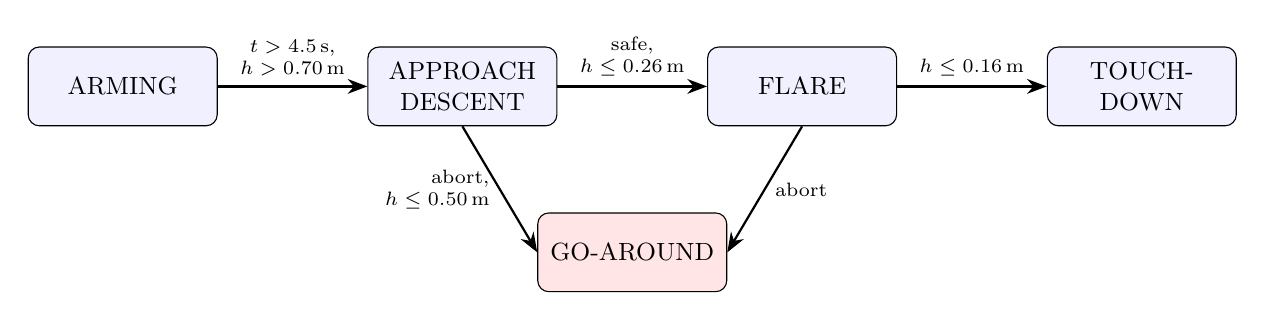
\begin{tikzpicture}[
  st/.style={draw,rounded corners,minimum width=2.4cm,minimum height=1.0cm,align=center,fill=blue!6,font=\small},
  arr/.style={-{Stealth[length=2.5mm]},thick}
]
\node[st] (a) {ARMING};
\node[st,right=1.9cm of a] (p) {APPROACH\\DESCENT};
\node[st,right=1.9cm of p] (f) {FLARE};
\node[st,right=1.9cm of f] (t) {TOUCH-\\DOWN};
\node[st,below=1.6cm of $(p)!0.5!(f)$,fill=red!10] (g) {GO-AROUND};
\draw[arr] (a) -- node[above,font=\scriptsize,align=center]{$t>4.5$\,s,\\$h>0.70$\,m} (p);
\draw[arr] (p) -- node[above,font=\scriptsize,align=center]{safe,\\$h\le0.26$\,m} (f);
\draw[arr] (f) -- node[above,font=\scriptsize,align=center]{$h\le0.16$\,m} (t);
\draw[arr] (p.south) -- node[left,font=\scriptsize,pos=0.5,align=right]{abort,\\$h\le0.50$\,m} (g.west);
\draw[arr] (f.south) -- node[right,font=\scriptsize,pos=0.5]{abort} (g.east);
\end{tikzpicture}
\caption{States of the approach supervisor. The go-around state has no exit transition in the implementation.}
\label{fig:flightfsm}
\end{figure}

\noindent
In \textsc{arming} the pitch setpoint is $0$ and the gear is stowed. The machine arms only after 4.5\,s of simulated time have elapsed (spawn settling) and the vehicle is confirmed airborne ($h>0.70$\,m). In \textsc{approach descent} the setpoint is a shallow descent attitude and the gear stays stowed above the decision height $H_{\mathrm{DH}}=0.50$\,m. At or below the decision height an abort leads immediately to a go-around, whereas a clear abort flag issues the deploy request and the approach continues; at the flare height the machine enters \textsc{flare} with a small nose-up setpoint. An abort during the flare also leads to a go-around. At the touchdown height the machine enters \textsc{touchdown}, the setpoint returns to zero, the gear remains deployed and the touchdown flag stops the motion. In \textsc{go-around} the setpoint becomes a climb attitude and the gear is stowed. The interlock of \cref{sec:gear} remains active in parallel: the gear controller forces the stowed angle whenever the abort flag is set.
 
\begin{table}[ht]
\centering
\small
\begin{tabular}{@{}L{5.6cm} l L{5.2cm}@{}}
\toprule
\textbf{Parameter} & \textbf{Value} & \textbf{Role}\\
\midrule
Descent pitch setpoint & $-0.045$\,rad & \textsc{approach descent}\\
Flare pitch setpoint & $+0.050$\,rad & \textsc{flare}\\
Climb pitch setpoint & $+0.200$\,rad & \textsc{go-around}\\
Decision height $H_{\mathrm{DH}}$ & 0.50\,m & Abort check and gear deployment\\
Flare height & 0.26\,m & Start of \textsc{flare}\\
Touchdown height & 0.16\,m & Start of \textsc{touchdown}\\
Arming conditions & $t>4.5$\,s, $h>0.70$\,m & Leaves \textsc{arming}\\
\bottomrule
\end{tabular}
\caption{Parameters of the approach supervisor (all except the arming conditions are ROS~2 parameters).}
\label{tab:supparams}
\end{table}
 
\paragraph{Known interface fault.} The attitude estimator publishes a stamped vector, whereas the supervisor subscribes with an unstamped vector type, so the supervisor does not receive the pitch estimate. The pitch value is not used in its state decisions, which depend on ground clearance, the abort flag and time, so the behaviour described here is unaffected, but the subscription is ineffective.
 
\paragraph{Approach testbed and carrier.} The approach scenario uses a fourth world that places the three terrain types in sequence along a 180\,m corridor: irregular vegetation mounds between $x=5$ and $25$\,m, a $20^\circ$ ramp (2.2\,m long, centred at $x=40$\,m) followed by a 0.20\,m stepped curb at $x=48$\,m, and a clear runway section from $x=58$ to $110$\,m. The airframe is not flown by aerodynamic forces: it is mounted on two position-controlled prismatic joints (a flight rail), and a carrier script commands its motion. The carrier advances along $x$ at 3.0\,m/s, holds a clearance of 0.85\,m up to $x=25$\,m, then descends linearly at 0.0115\,m per metre travelled down to 0.16\,m, climbs at 0.60\,m/s up to 3\,m when the pitch setpoint exceeds 0.10\,rad (go-around), and stops at touchdown. The supervisor therefore decides, but the trajectory is prescribed, and the pitch loop of \cref{sec:pid} acts on a vehicle whose body motion is not coupled to the stabilator. A simplified pitching-moment node exists in the source tree but is not launched.
 
 
 
%==============================================================
\section{Software Implementation}\label{sec:impl}
%==============================================================
\subsection{Platform}
The system is implemented for Ubuntu~24.04 with ROS~2 Jazzy Jalisco~\cite{ros2} and Gazebo Harmonic~\cite{gazebo}. The domain nodes are written in C++ and built with \code{colcon}; the data-collection, training and verification tools are Python scripts. A bridge maps Gazebo topics to ROS~2, and a launch file starts the simulator (with or without GUI), spawns the airframe in the selected world and starts all nodes with simulation time enabled. The static verification uses the launch option that disables the flight mode.
 
\subsection{Nodes}
\begin{table}[ht]
\centering
\small
\begin{tabular}{@{}L{4.3cm} L{2.0cm} L{5.6cm} L{2.4cm}@{}}
\toprule
\textbf{Node} & \textbf{Domain} & \textbf{Function} & \textbf{Rate}\\
\midrule
\code{sensor\_processor} & Sensing & Range extraction, slope, variances, features (\cref{alg:features}) & 20\,ms timer (nominal 50\,Hz)\\
\code{terrain\_classifier} & Intelligence & Compiled tree inference, verdict, abort & per feature message\\
\code{attitude\_estimator} & Control & Complementary filter (\cref{alg:cf}) & per IMU message (100\,Hz)\\
\code{stabilator\_controller} & Control & PID pitch stabilisation (\cref{alg:pid}) & per attitude message (100\,Hz)\\
\code{landing\_gear\_controller} & Control & Interlocked, rate-limited gear (\cref{alg:gear}) & 50\,Hz\\
\code{flight\_supervisor} & Control & Approach state machine (\cref{sec:supervisor}) & 20\,ms timer (nominal 50\,Hz)\\
\code{flight\_carrier} (script) & Simulation & Prescribed flight-rail trajectory & 50\,Hz\\
\bottomrule
\end{tabular}
\caption{ROS~2 nodes of the simulation. The last two nodes belong to the approach scenario.}
\label{tab:nodes}
\end{table}
 
\subsection{Interfaces}
The principal topics are listed in \cref{tab:topics}. Raw sensor streams and the sensing node's inputs use the sensor-data quality of service (best effort) to favour freshness over delivery guarantees; processed and control topics use reliable delivery. A queue depth of ten does not make a topic latched, so a late-joining subscriber does not receive earlier values of the deploy request or pitch setpoint. The coordinate frames and sensor poses are defined in the rig description of the repository.
 
\begin{table}[ht]
\centering
\small
\begin{tabular}{@{}L{4.6cm} L{3.7cm} L{1.9cm} L{3.7cm}@{}}
\toprule
\textbf{Topic} & \textbf{Type} & \textbf{Rate} & \textbf{Purpose}\\
\midrule
\code{/sensing/imu/data\_raw} & \code{sensor\_msgs/Imu} & 100\,Hz & Raw accelerations and rates\\
\code{/sensing/tof/*} & \code{sensor\_msgs/LaserScan} & nominal 50\,Hz & Optical ranges (three)\\
\code{/sensing/sonar/scan} & \code{sensor\_msgs/LaserScan} & 20\,Hz (model) & Acoustic ranges\\
\code{/sensing/altitude\_agl} & \code{Float64} & nominal 50\,Hz & Mean ToF range\\
\code{/sensing/features} & \code{Float32MultiArray} & nominal 50\,Hz & Seven-element feature vector\\
\code{/intelligence/verdict} & \code{Int32} & per feature & 0 safe, 1 slope, 2 vegetation\\
\code{/intelligence/abort} & \code{Bool} & per feature & Interlock override\\
\code{/control/attitude} & \code{Vector3Stamped} & 100\,Hz & Filtered roll and pitch\\
\code{/control/pitch\_setpoint} & \code{Float64} & nominal 50\,Hz & Pitch reference (supervisor)\\
\code{/control/elevator\_cmd} & \code{Float64} & 100\,Hz & Stabilator command\\
\code{/control/gear\_deploy} & \code{Bool} & nominal 50\,Hz & Deploy request\\
\code{/control/gear\_cmd}, \code{gear\_status} & \code{Float64} & 50\,Hz & Rate-limited gear command and status\\
\code{/flight/touchdown} & \code{Bool} & nominal 50\,Hz & Touchdown flag\\
\code{/flight/supervisor\_state} & \code{String} & nominal 50\,Hz & State label\\
\bottomrule
\end{tabular}
\caption{Selected ROS~2 topics. Nominal rates are those of the timers or of the simulated sensors; they were not measured.}
\label{tab:topics}
\end{table}
 
\section{Hardware Bench Prototype}\label{sec:bench}
%==============================================================
In addition to the simulation, a physical bench prototype implements a subset of the same sensing and control ideas on real sensors~\cite{repo}. Its purpose is to exercise attitude estimation, a stabiliser command, landing-readiness checks and a gear sequence on measured data, not to classify terrain. It is a deliberately reduced build: all functions run on one Arduino Uno, only one range sensor is connected, and both actuators are virtual, that is, the firmware computes and reports the commanded angles but drives no servo.
 
\subsection{Hardware and connections}
The connected hardware is listed in \cref{tab:benchhw}. The IMU is an MPU6500 breakout (GY-6500) configured at I$^2$C address \code{0x68}, and the ToF sensor is a regulated VL53L0X breakout~\cite{vl53} at its default address \code{0x29}. Both modules share the Uno's 3.3\,V supply, ground and I$^2$C bus (\cref{tab:wiring}); the bus runs at 400\,kHz with a bounded transaction timeout (where the library supports it) so that a stuck transfer cannot block the control loop. The VDD, XSHUT and GPIO1 pins of the ToF breakout are left unconnected. Both SG90 servos remain disconnected because no suitable actuator supply is available, and the firmware's actuator output routine is deliberately empty.
 
\begin{table}[ht]
\centering
\small
\begin{tabular}{@{}L{4.2cm} L{10.5cm}@{}}
\toprule
\textbf{Component} & \textbf{Role}\\
\midrule
Arduino Uno & Acquisition, attitude estimation, readiness checks and virtual commands (sensing, intelligence and control on one board)\\
GY-6500 / MPU6500 IMU~\cite{mpu6500} & Three-axis acceleration and angular rate\\
One VL53L0X breakout & Sensor-to-target distance and measurement status\\
Breadboard, jumper wires & Shared power, ground and I$^2$C connections\\
USB link to a computer & Power, firmware upload and serial monitoring\\
\bottomrule
\end{tabular}
\caption{Connected hardware of the bench prototype.}
\label{tab:benchhw}
\end{table}
 
\begin{table}[ht]
\centering
\small
\begin{tabular}{@{}l l l@{}}
\toprule
\textbf{Uno} & \textbf{MPU6500 module} & \textbf{VL53L0X breakout}\\
\midrule
3.3\,V & Power input & VIN\\
GND & GND & GND\\
A4 (SDA) & SDA & SDA\\
A5 (SCL) & SCL & SCL\\
\bottomrule
\end{tabular}
\caption{Wiring of the one-ToF bench setup.}
\label{tab:wiring}
\end{table}
 

\noindent
The ESP32, the ultrasonic sensors, the magnetometer and additional ToF sensors are not used. The firmware contains a prepared three-ToF configuration (individual shutdown pins and re-assigned I$^2$C addresses) that is disabled; enabling it requires a suitable power arrangement, bus-voltage compatibility, individual shutdown wiring and a rigid sensor geometry, so it is not a working three-sensor terrain estimator. In particular, a single beam measures the range to a target and cannot give slope, surface material or a tilt-corrected altitude.
 
\subsection{Attitude estimation and virtual stabiliser}
\paragraph{Calibration.} At start-up the IMU must be level and stationary with its $+z$ axis pointing upward. The driver estimates accelerometer and gyroscope biases, which are held in RAM and recomputed after every reset; start-up takes about 20\,s plus sensor initialisation. The driver reports acceleration in units of $g$ and angular rate in degrees per second, so the accelerometer angles are formed from ratios without a conversion to m/s$^2$.
 
\paragraph{Complementary filter with measured time step.} The firmware samples at a nominal 100\,Hz and uses the elapsed time $\Delta t_k$ between samples, measured with the microsecond timer, instead of a fixed period. The accelerometer angles are
\begin{equation}
\phi_{\mathrm{acc}}=\operatorname{atan2}(a_y,a_z),\qquad
\theta_{\mathrm{acc}}=\operatorname{atan2}\!\bigl(-a_x,\sqrt{a_y^2+a_z^2}\bigr),
\end{equation}
and the filter weight is derived from a fixed time constant $\tau=0.50$\,s,
\begin{equation}
\alpha_k=\frac{\tau}{\tau+\Delta t_k},\qquad
\theta_k=\alpha_k\bigl(\theta_{k-1}+\omega_y\,\Delta t_k\bigr)+(1-\alpha_k)\,\theta_{\mathrm{acc}},
\label{eq:cfbench}
\end{equation}
with the roll channel handled in the same way and angles wrapped to $\pm180^\circ$. Because $\alpha_k$ follows $\Delta t_k$, timing jitter does not change the time constant of the filter. At 100\,Hz, $\alpha\approx0.980$ and the corner frequency is $1/(2\pi\tau)\approx0.32$\,Hz, which is lower than in the simulation ($\alpha=0.9$, $\tau\approx0.095$\,s, about 1.7\,Hz): the bench filter trusts the gyroscope for longer and therefore reacts more slowly to the accelerometer, which suppresses vibration and hand-motion noise at the cost of a slower correction of gyroscope drift. The estimate is initialised from the accelerometer at the actual tilt, and is re-initialised whenever the gap between samples exceeds 0.20\,s, because the motion during the missing interval was not observed. A sample is rejected as invalid if any value is non-finite or the acceleration magnitude is practically zero ($|\vect a|^2<10^{-6}\,g^2$); the filter state is then discarded and restarted at the next valid sample. Single precision is used throughout, which also avoids the integer overflow discussed in \cref{sec:attitude}.
 
\paragraph{Virtual stabiliser command.} The stabiliser command is a proportional response to the pitch error,
\begin{equation}
u=\operatorname{clamp}\bigl(90^\circ+K\,e,\ 65^\circ,\ 115^\circ\bigr),\qquad e=\begin{cases}0,&|\theta_{\mathrm{ref}}-\hat\theta|\le1^\circ\\[2pt]\theta_{\mathrm{ref}}-\hat\theta,&\text{otherwise,}\end{cases}
\label{eq:vstab}
\end{equation}
with $K=1$ degree of servo angle per degree of pitch error, $\theta_{\mathrm{ref}}=0$, a neutral angle of $90^\circ$ and a travel of $\pm25^\circ$, the same authority as the simulated stabilator. A pitch of $+10^\circ$ therefore produces a command of $80^\circ$, which opposes the tilt in the sense assumed for the mechanism; the sign of $K$ must be verified against the real linkage before a servo is connected. The $\pm1^\circ$ deadband prevents the command from dithering around the neutral angle. If the IMU sample is invalid, the stabiliser command returns to $90^\circ$ while a deployed gear command is retained. There is no integral or derivative action, no aerodynamic plant and no servo feedback: the command is displayed, not applied, and the demonstration shows the response to hand tilt, which does not prove physical stabilisation.
 
\subsection{One-ToF landing-readiness rules}\label{sec:readiness}
The readiness logic replaces the terrain classifier of the simulation with a short set of measured rules (\cref{tab:rules}). The ToF sensor runs in continuous mode with a nominal 50\,ms period, and a new distance is entered into the stability window only when a distinct new result is read; polling an existing result does not count as a new sample. A reading is valid if the sensor is available, the bus transfer succeeded, the device status is valid and the result is at most 250\,ms old.
 
\begin{table}[ht]
\centering
\small
\begin{tabular}{@{}L{4.6cm} L{10.1cm}@{}}
\toprule
\textbf{Check} & \textbf{Demonstration setting}\\
\midrule
Sensor-to-target distance & 100 to 500\,mm, inclusive\\
Absolute pitch and roll & At most $10^\circ$ each\\
Stability window & Ten completed, valid ToF measurements\\
Distance spread in the window & $\max-\min\le20$\,mm, all samples inside the distance limits\\
Range freshness & At most 250\,ms since the last result\\
Qualification time & All checks continuously satisfied for 1\,s after the window is complete\\
\bottomrule
\end{tabular}
\caption{Landing-readiness rules of the bench prototype. The values are configurable demonstration settings, not aircraft operating limits.}
\label{tab:rules}
\end{table}

\noindent
The status is one of three values. \textsc{unknown} means that data are missing, invalid or still being collected or qualified; \textsc{unsafe} means that a measured rule has failed; \textsc{ready} means that all rules have been satisfied for the qualification time (\cref{alg:ready}). A fault or a stale result empties the whole window, whereas a failed tilt, distance or spread check restarts only the qualification timer. No hysteresis is implemented, so the one-second qualification is the only mechanism that delays re-entry into \textsc{ready}.
 
\begin{algorithm}[ht]
\caption{Landing-readiness evaluation (every control cycle)}\label{alg:ready}
\begin{algorithmic}[1]
\Require attitude validity, pitch $\theta$, roll $\phi$, ToF reading (distance $d$, validity, age), window $W$ of the last ten distances
\Ensure status $\in\{\textsc{unknown},\textsc{unsafe},\textsc{ready}\}$
\If{attitude invalid \textbf{or} ToF reading invalid \textbf{or} age $>250$\,ms}
  \State clear $W$ and the qualification timer; \Return \textsc{unknown}
\EndIf
\If{$|\theta|>10^\circ$ \textbf{or} $|\phi|>10^\circ$} \State restart timer; \Return \textsc{unsafe} \EndIf
\If{$d<100$\,mm \textbf{or} $d>500$\,mm} \State restart timer; \Return \textsc{unsafe} \EndIf
\If{$|W|<10$} \State restart timer; \Return \textsc{unknown} \EndIf
\If{$\max W-\min W>20$\,mm \textbf{or} any $w\in W$ outside $[100,500]$\,mm}
  \State restart timer; \Return \textsc{unsafe}
\EndIf
\If{timer not running} \State start timer \EndIf
\If{timer $<1$\,s} \State \Return \textsc{unknown} \Comment{qualifying}
\EndIf
\State \Return \textsc{ready}
\end{algorithmic}
\end{algorithm}
 
\subsection{Latched gear sequence}\label{sec:benchgear}
Operator commands arrive over the serial link (\cref{tab:commands}). Deployment is accepted only while the status is \textsc{ready}; an early request is rejected with the current reason and is not queued. Once accepted, the virtual gear command is latched at $90^\circ$ and stays latched when distance, tilt or sensor validity change: the report then shows a warning and the current readiness reason, and the gear is released only by an explicit stow command or a board reset, which starts stowed. Readiness is evaluated independently of the gear state, so the gear can be deployed while the status is \textsc{unknown} or \textsc{unsafe}. After readiness has been lost, a fresh qualification is required before a new deployment can be accepted, and nothing deploys automatically. All displayed angles are commands, not measured positions.
 
\begin{table}[ht]
\centering
\small
\begin{tabular}{@{}l L{12.2cm}@{}}
\toprule
\textbf{Command} & \textbf{Behaviour}\\
\midrule
\code{D} & Deploy the virtual gear to $90^\circ$ while \textsc{ready}; otherwise reject with a reason\\
\code{S} & Stow the virtual gear at $0^\circ$, also during sensor faults\\
\code{M} & Readable serial reports at 2\,Hz (default)\\
\code{V} & Raw six-value IMU frames at 20\,Hz for the desktop viewer\\
\bottomrule
\end{tabular}
\caption{Serial commands of the bench prototype (lower case is also accepted).}
\label{tab:commands}
\end{table}
 
\paragraph{Contrast with the simulated interlock.} The two prototypes use opposite policies once the gear is down. In the simulation (\cref{sec:gear}) an unsafe verdict forces the gear to the stowed position, so that deployment is always subordinate to the classifier. In the bench prototype a deployed gear is held until the operator stows it, because the commands are virtual and the loss of a single-beam range reading, which may be caused by the target leaving the field of view, is not evidence of a hazard. The policies differ intentionally, and neither one establishes flight safety.
 
\subsection{Firmware and desktop tools}
The firmware is a single Arduino sketch that uses the FastIMU~\cite{fastimu} and Pololu VL53L0X~\cite{pololu} libraries and communicates at 115\,200\,baud. A cooperative loop runs once per 10\,ms sample interval: it reads the IMU, updates the attitude, polls the ToF sensor, evaluates the readiness rules, then processes at most sixteen command characters against these fresh readings, computes the virtual commands and, at the selected interval, emits telemetry. Unsigned subtraction of the microsecond timer remains correct across counter roll-over. Fixed text is held in flash memory so that the 2\,kB of RAM of the ATmega328P are not consumed by strings. The readable report contains the gear sequence, the readiness status and its reason, pitch and roll, the range and its status, the stability-window progress, the actuator command angles and warnings.
\\
\noindent 
A Python desktop application (Tkinter and \code{pyserial}) connects to the Uno, shows the report or a raw IMU view with a ten-sample moving average that affects only the display, and sends the deploy and stow commands; the firmware alone decides whether a deployment is allowed. Viewer frames use the format \code{S<ax>/<ay>/<az>/<gx>/<gy>/<gz>E}, one per line, and non-finite or malformed frames are rejected. Opening the serial port can reset the board, so the IMU must be kept level during the start-up calibration, and only one application can own the port at a time. Automated unit tests with a mocked serial connection cover frame parsing and finite-value validation, display averaging, fragmented input, serial errors and the integration of display and commands; they need no hardware.
 
\subsection{Demonstration checks}
The expected behaviour of the bench prototype for the demonstration scenarios is summarised in \cref{tab:benchchecks}. The connected setup and its serial reports were exercised on hardware, but no quantitative characterisation (for example of timing, range accuracy or attitude error against a reference) was carried out, and the readiness thresholds are provisional.
 
\begin{table}[ht]
\centering
\small
\begin{tabular}{@{}L{6.2cm} L{8.6cm}@{}}
\toprule
\textbf{Scenario} & \textbf{Expected behaviour}\\
\midrule
Level IMU, stable target inside the range window & \textsc{ready} after ten readings and one second of qualification\\
Deploy before \textsc{ready} & Rejected with a reason; the request is not saved\\
Deploy while \textsc{ready} & Gear command becomes deployed at $90^\circ$\\
Change distance or tilt after deployment & Readiness changes; the deployed command stays latched with a warning\\
Remove the target or interrupt ToF communication & \textsc{unknown}, stability window reset, deployed command retained\\
Restore acceptable readings & Fresh qualification is required; no automatic deployment\\
Stow command & Gear command becomes stowed at $0^\circ$\\
Tilt the IMU about its $y$ axis & Stabiliser command reacts to pitch and respects its limits\\
\bottomrule
\end{tabular}
\caption{Demonstration scenarios and expected behaviour of the bench prototype.}
\label{tab:benchchecks}
\end{table}
 
\paragraph{Limits of the bench prototype.} The prototype has no servo-position feedback, touchdown detection, yaw estimate, aerodynamic feedback or automatic landing control. Translational acceleration distorts the gravity reference of the accelerometer, and the gyroscope integration is intended for moderate bench tilts. The numeric validation of IMU samples cannot detect every plausible stale reading, and the ToF validation uses the raw device status rather than the full quality assessment of the manufacturer's software. A single beam cannot establish terrain slope or surface material, so a \textsc{ready} status expresses only that the configured bench conditions hold and must not be read as a terrain-safety classification.
 
 
%==============================================================
\section{Verification and Validation of the Simulation}\label{sec:validation}
%==============================================================
\subsection{Synthetic testbeds}
Four Gazebo worlds provide the terrain (\cref{tab:worlds}). The first three are static: the rig stands on a fixed mount 0.70\,m above the ground, so only the sensing, classification and gear chain is exercised. \Cref{fig:rig} shows the rig and \cref{fig:beta,fig:gamma} the Beta and Gamma worlds; the Alpha world is a flat ground plane and no screenshot of it is included. The fourth world places the three terrain types in sequence for the approach scenario (\cref{fig:approach}).
 
\begin{table}[ht]
\centering
\small
\begin{tabular}{@{}l L{8.0cm} l@{}}
\toprule
\textbf{World} & \textbf{Terrain} & \textbf{Label}\\
\midrule
Alpha & Flat ground plane & \textsc{safe} (0)\\
Beta & $20^\circ$ inclined ramp (a $4\times4$\,m slab) and a stepped curb block beside it & \textsc{unsafe\_slope} (1)\\
Gamma & Three box-shaped mounds and a central solid cylinder; no penetrable vegetation is modelled & \textsc{unsafe\_vegetation} (2)\\
Approach & Vegetation mounds ($x=5$ to 25\,m), a $20^\circ$ ramp (centred at $x=40$\,m), a curb ($x=48$\,m) and a runway ($x=58$ to 110\,m) & used by the supervisor\\
\bottomrule
\end{tabular}
\caption{Synthetic testbeds.}
\label{tab:worlds}
\end{table}
 
\begin{figure}[ht]
\centering
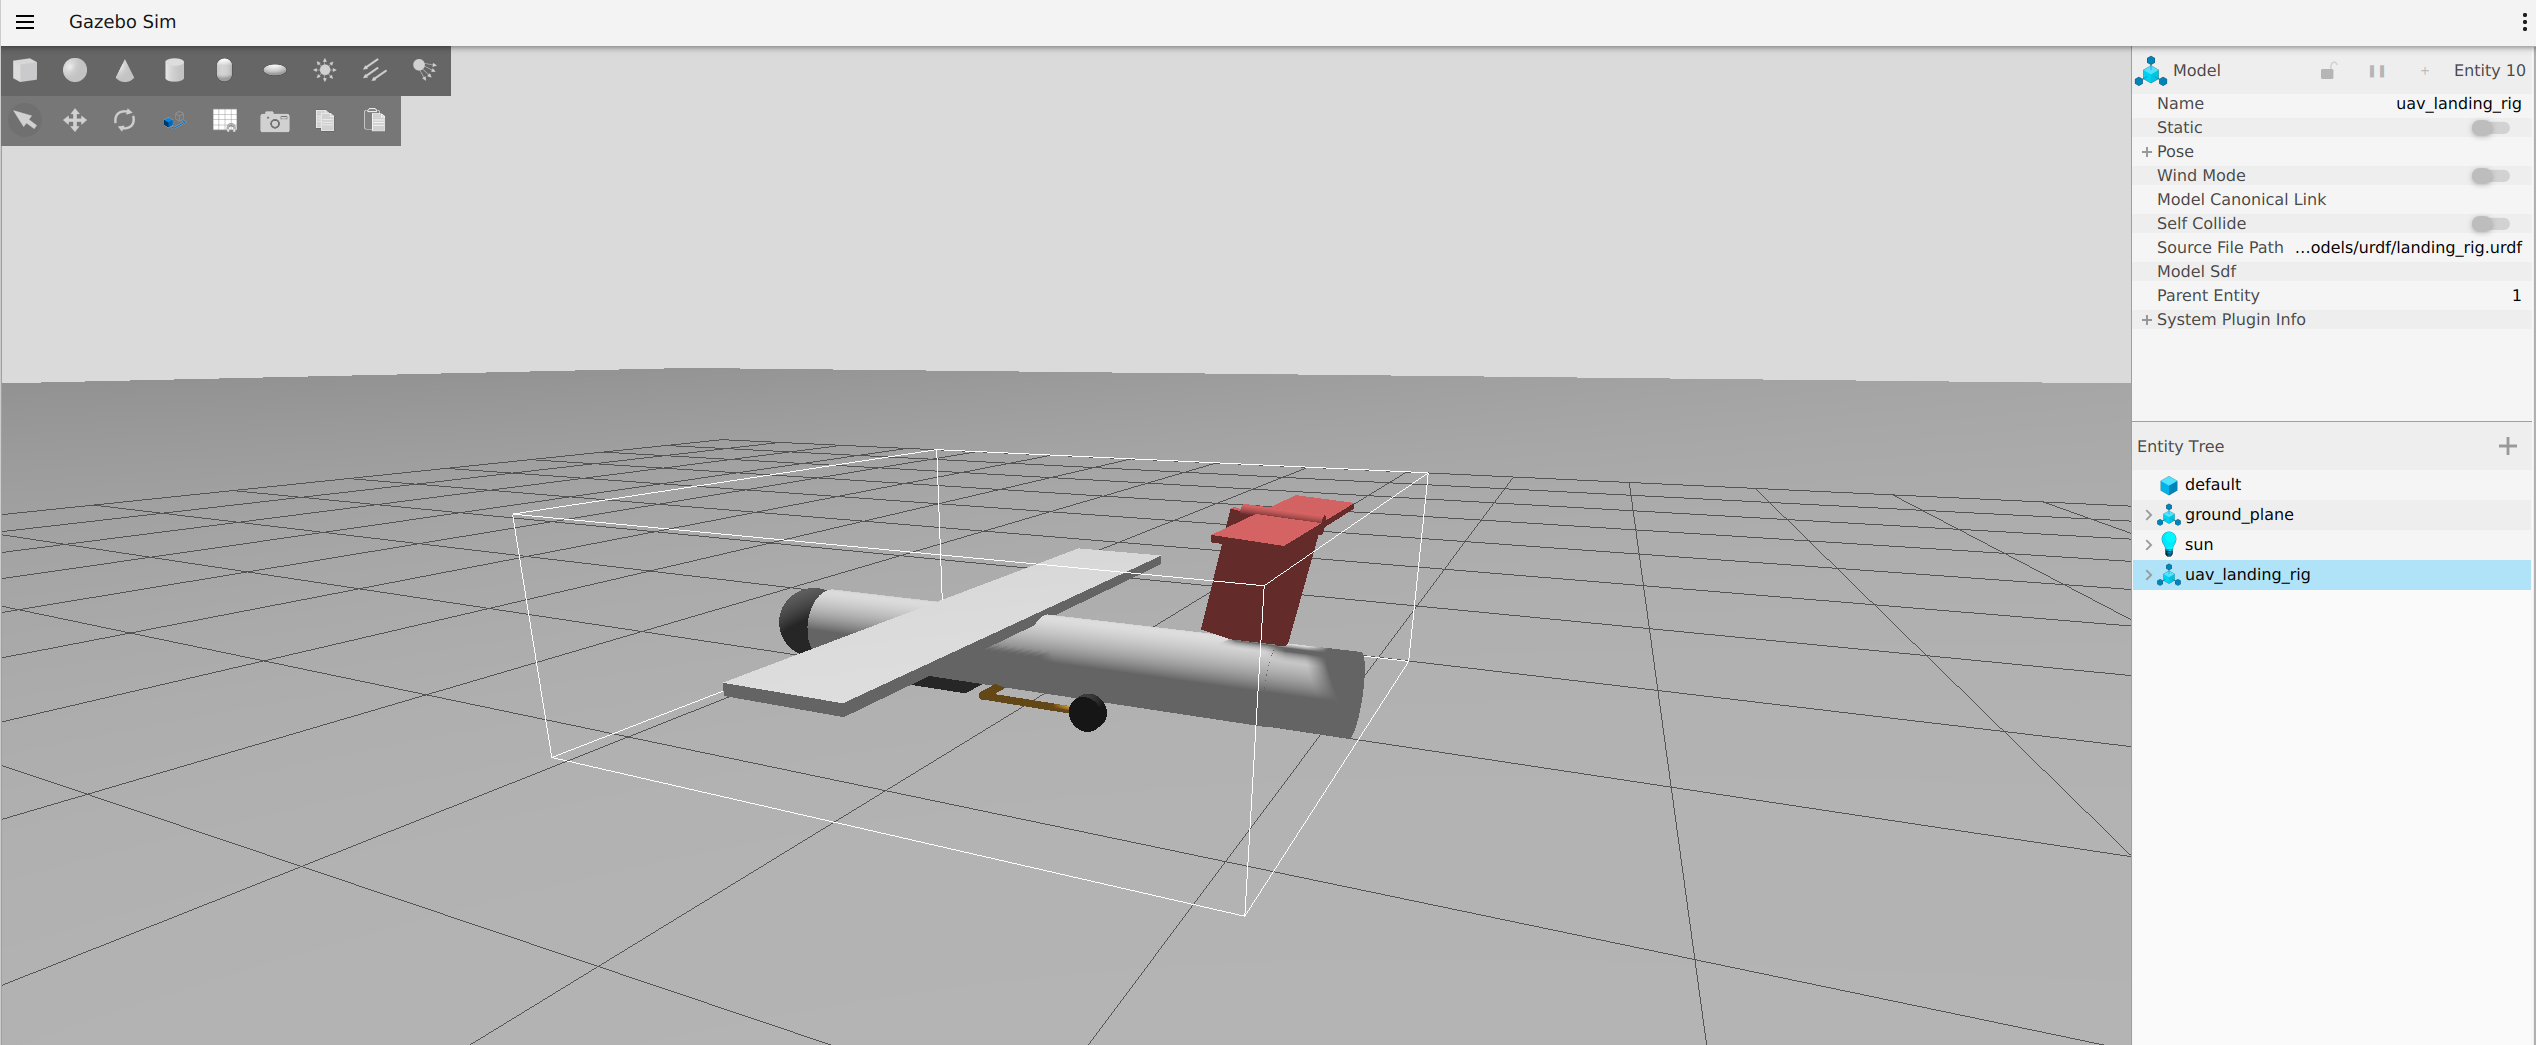
\includegraphics[width=0.92\linewidth]{figs/gazebo_rig_closeup.png}
\caption{Gazebo view of the simulated rig: fuselage with the ventral sensor plate, high wing, T-tail with the stabilator and the retractable gear.}
\label{fig:rig}
\end{figure}
 
\begin{figure}[ht]
\centering
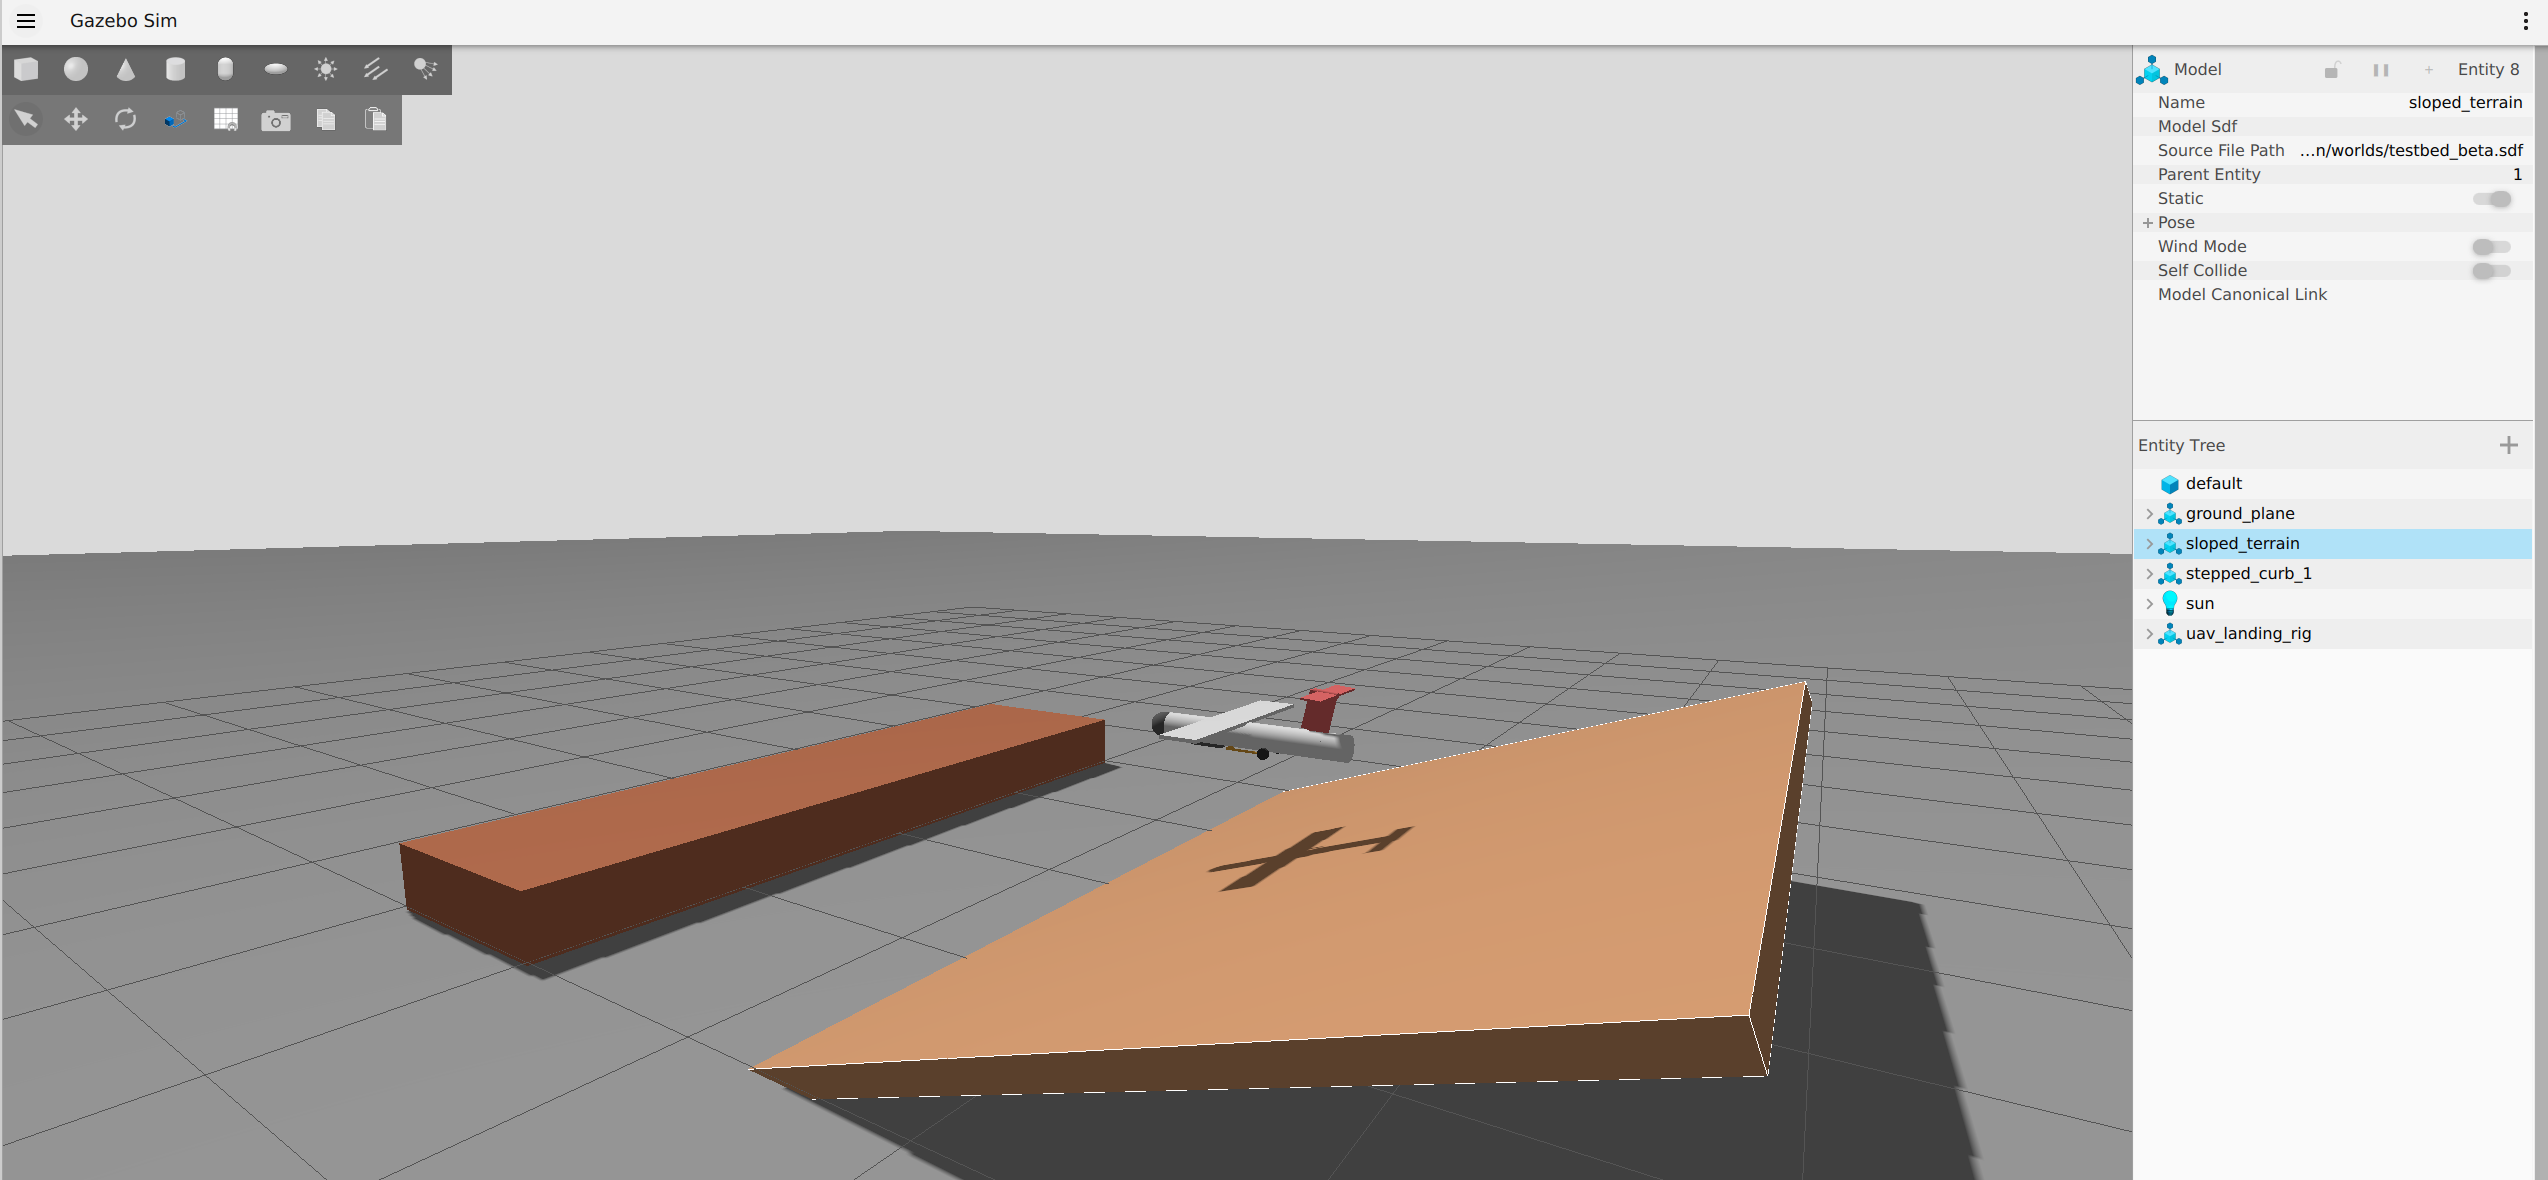
\includegraphics[width=0.92\linewidth]{figs/gazebo_beta_world.png}
\caption{Beta world: the rig on its stand beside the $20^\circ$ ramp slab (right) and the stepped curb block (left).}
\label{fig:beta}
\end{figure}
 
\begin{figure}[ht]
\centering
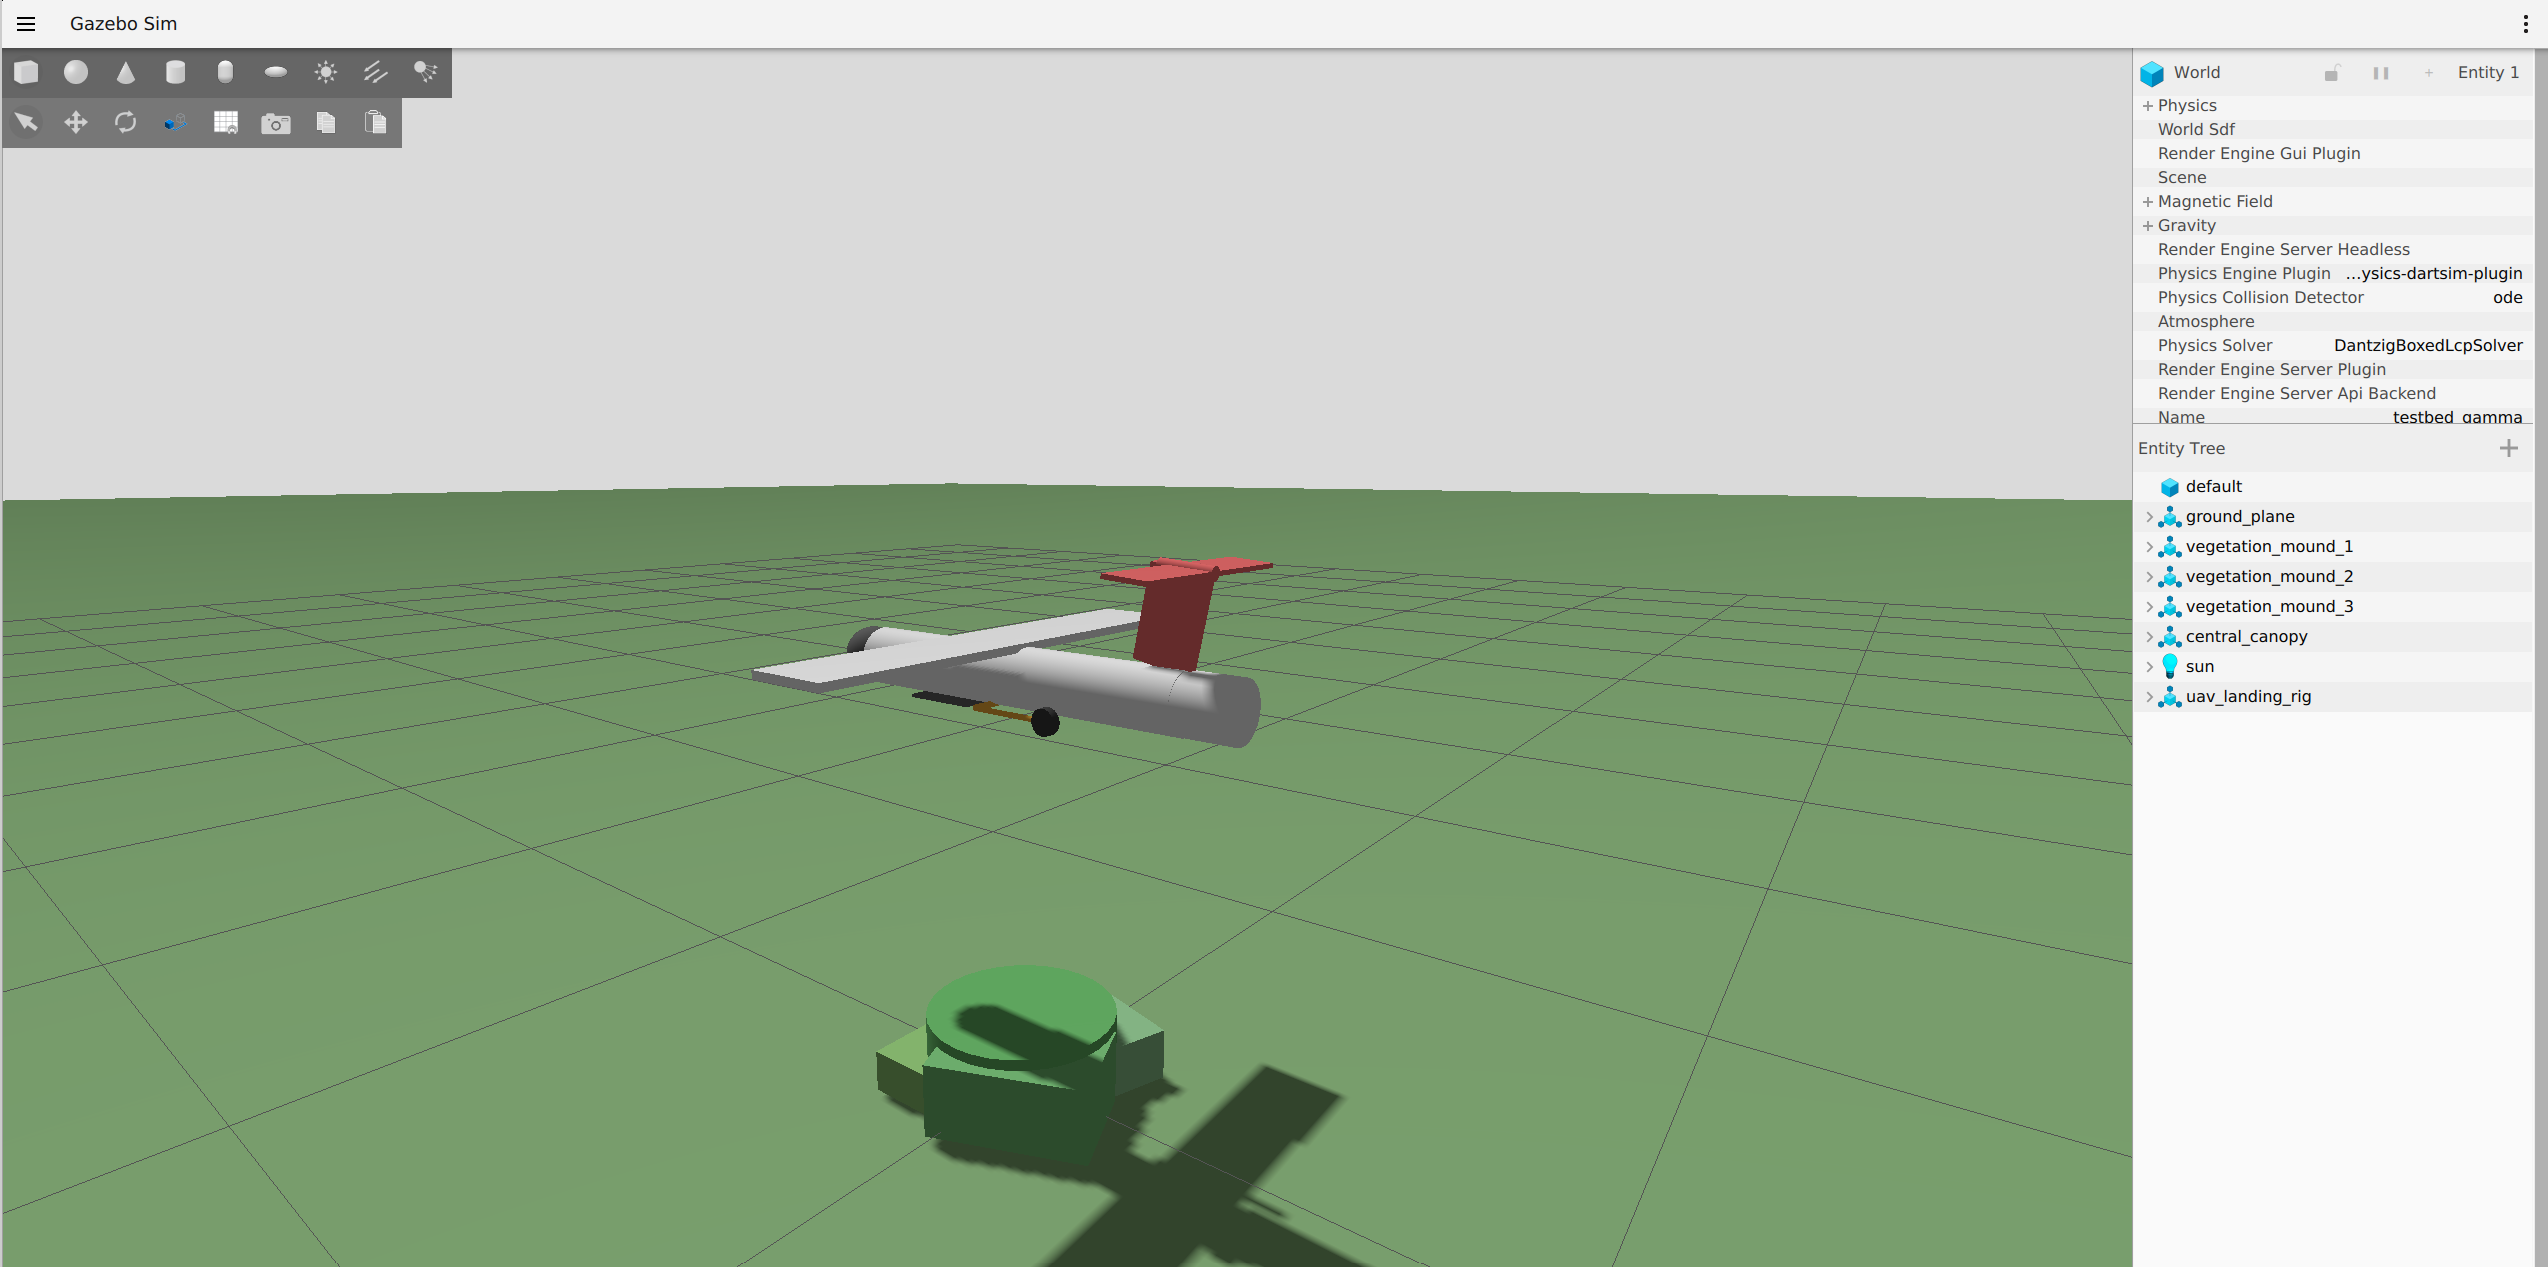
\includegraphics[width=0.92\linewidth]{figs/gazebo_gamma_world.png}
\caption{Gamma world: the rig above the mounds and the central cylinder.}
\label{fig:gamma}
\end{figure}
 
\begin{figure}[ht]
\centering
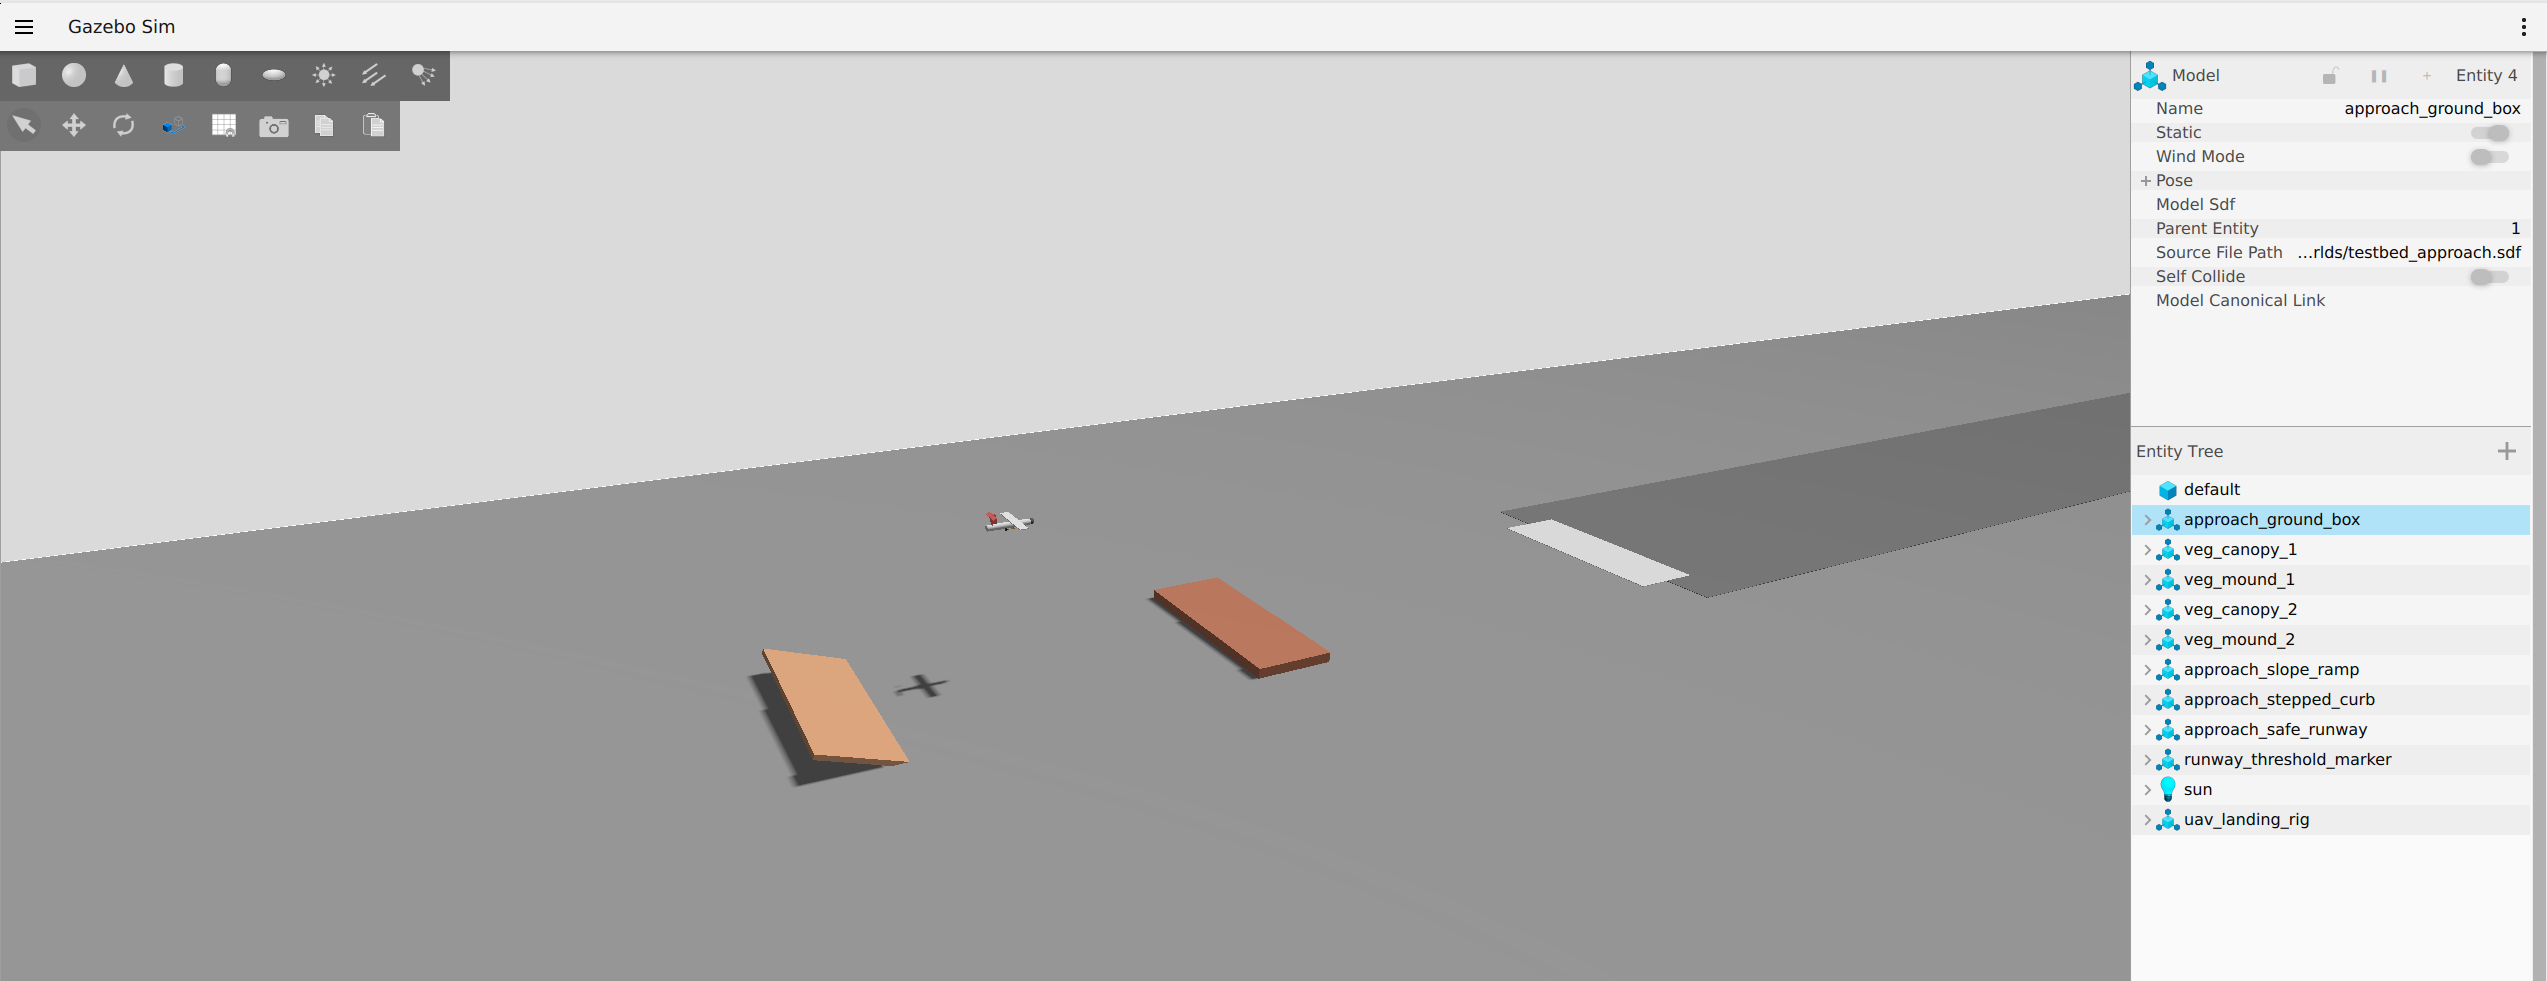
\includegraphics[width=0.92\linewidth]{figs/gazebo_approach_world.png}\\[4pt]
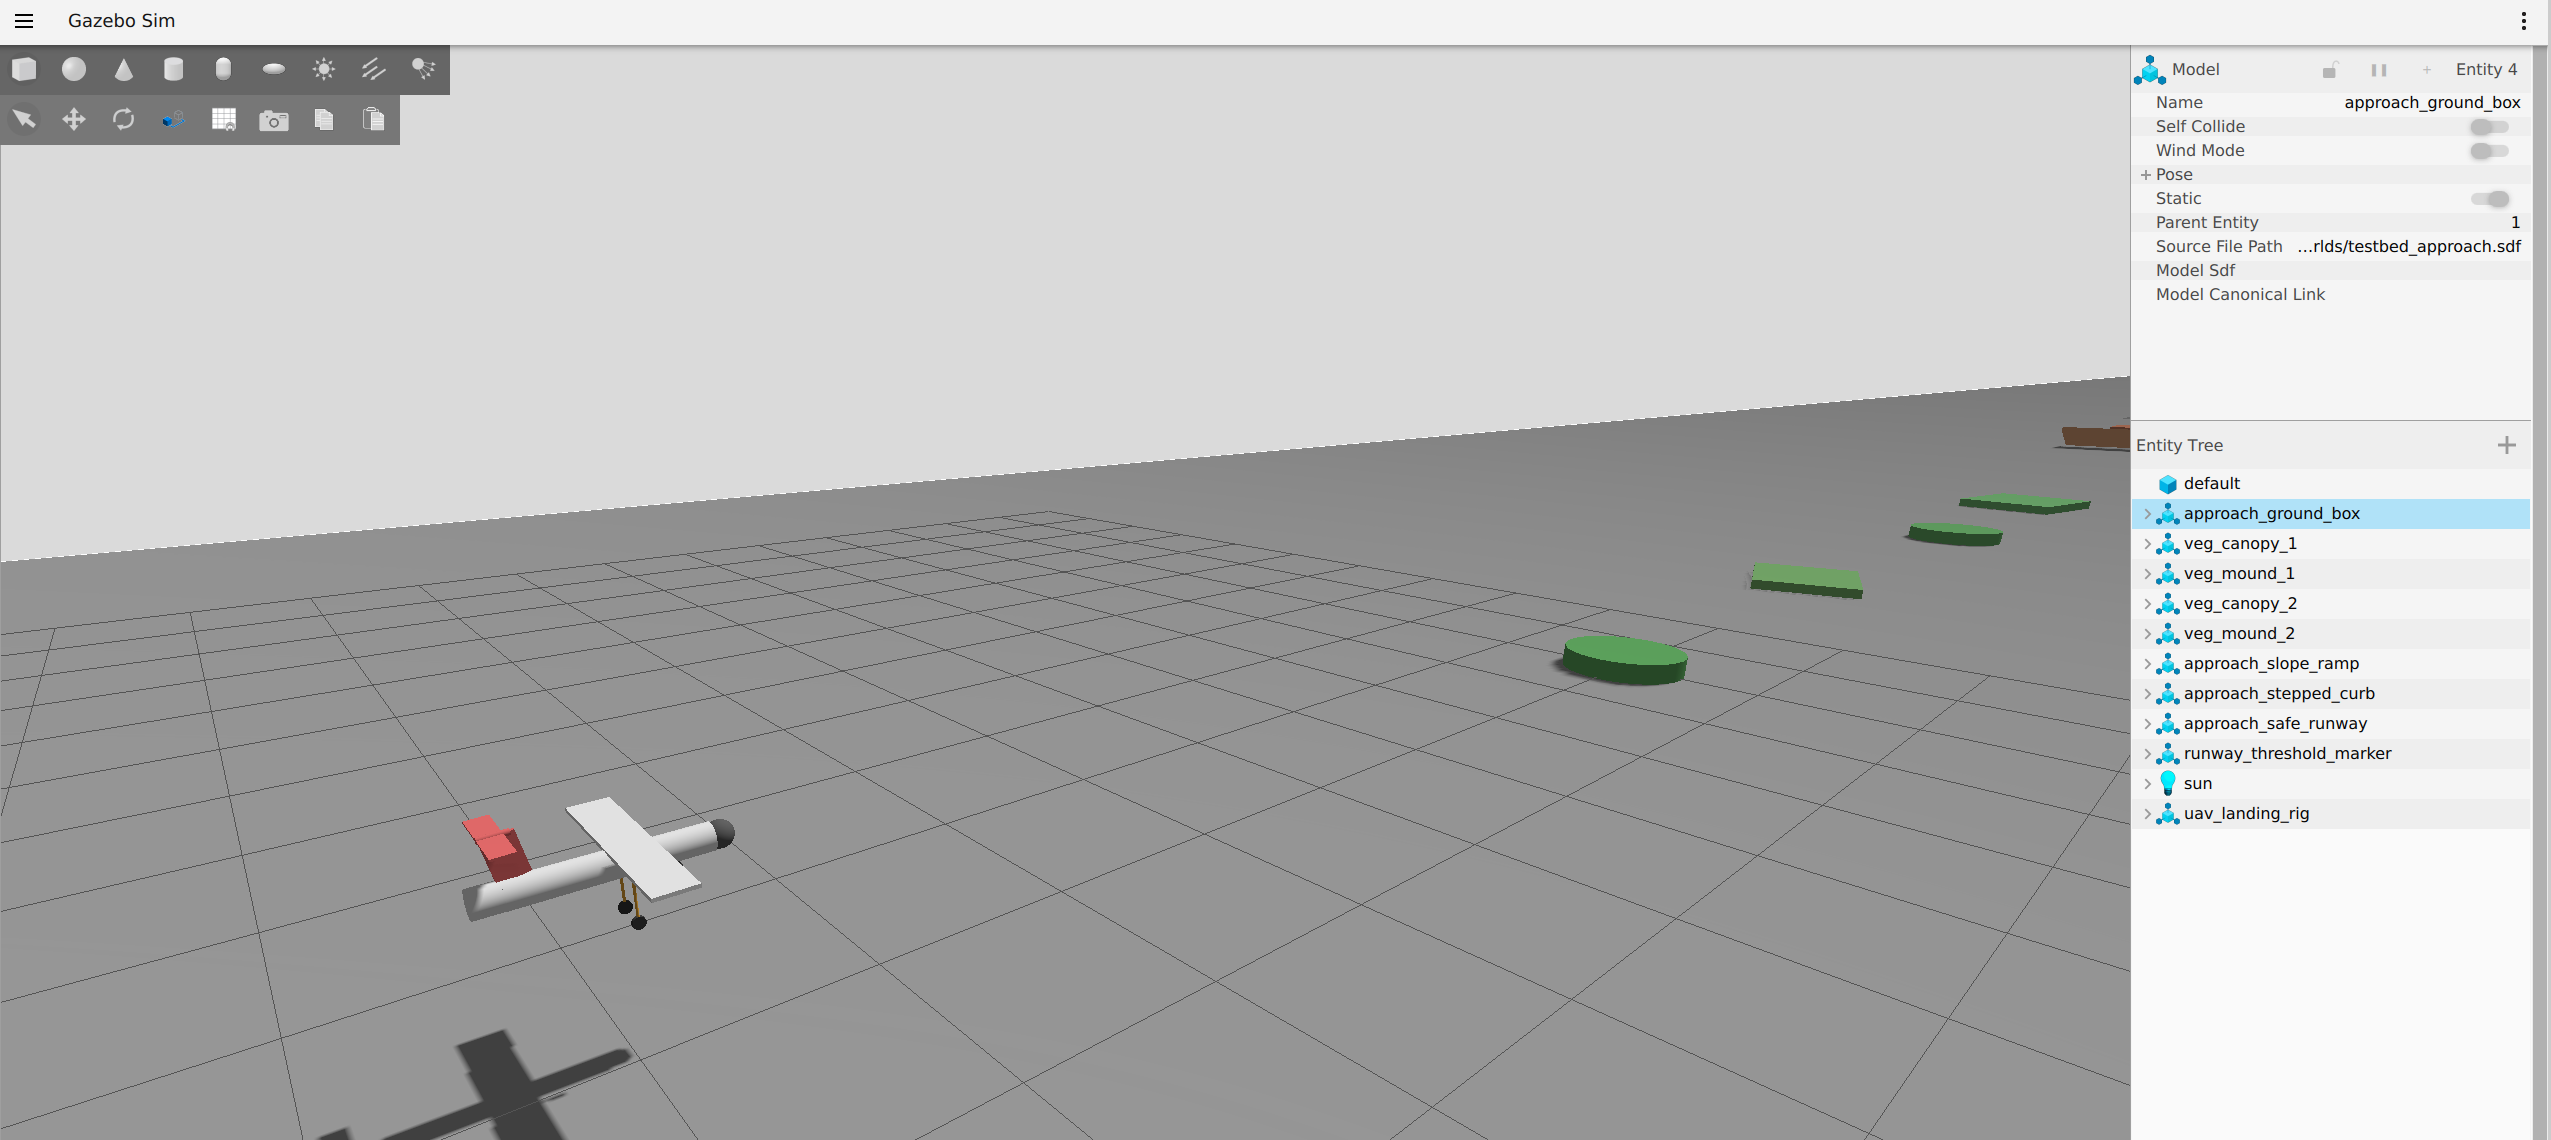
\includegraphics[width=0.92\linewidth]{figs/gazebo_approach_world_alt.png}
\caption{Approach world used with the supervisor: terrain sectors laid out along the flight corridor, seen from two viewpoints.}
\label{fig:approach}
\end{figure}
 
\subsection{Scenario verification}
The verification script launches each of Alpha, Beta and Gamma headlessly in static mode. It waits up to 60\,s for ten valid scans per range sensor and fresh feature, verdict, abort and gear telemetry, and requires one second of readiness. It then sends repeated deployment requests and waits up to 15\,s for the expected verdict, abort flag and gear status to hold for one second, and it writes a launch log for each world. Readiness failures are reported as failures, so fallback feature values cannot make a scenario pass. The script checks only the verdict, the abort flag and the gear status generated by the controller; it does not measure joint motion, and it does not cover the flying approach.
 
\begin{figure}[ht]
\centering
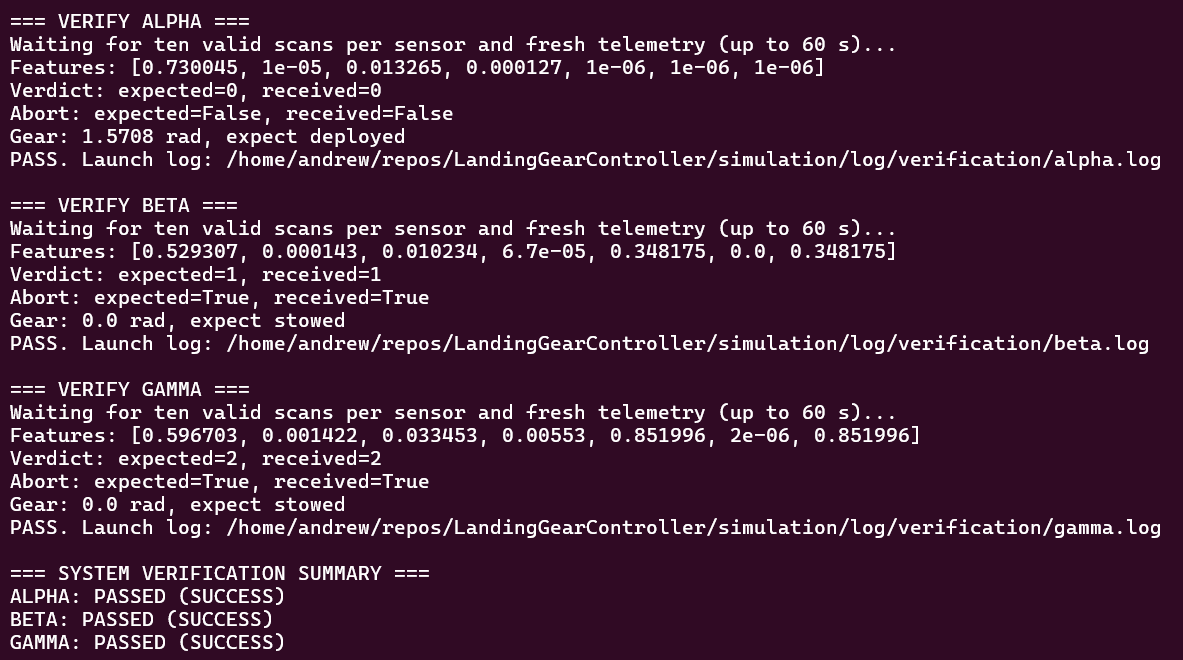
\includegraphics[width=0.85\linewidth]{figs/verify_system_output.png}
\caption{Terminal output of the verification script for the three static worlds.}
\label{fig:verify}
\end{figure}
 
\begin{table}[ht]
\centering
\small
\begin{tabular}{@{}l r r r@{}}
\toprule
\textbf{Quantity} & \textbf{Alpha} & \textbf{Beta} & \textbf{Gamma}\\
\midrule
0 Mean ToF range (m) & 0.730045 & 0.529307 & 0.596703\\
1 Spatial variance (m$^2$) & 0.00001 & 0.000143 & 0.001422\\
2 $\Delta d$ (m) & 0.013265 & 0.010234 & 0.033453\\
3 Sonar scan variance (m$^2$) & 0.000127 & 0.000067 & 0.00553\\
4 Total slope (rad) & 0.000001 & 0.348175 & 0.851996\\
5 Roll slope magnitude (rad) & 0.000001 & 0 & 0.000002\\
6 Total slope (rad) & 0.000001 & 0.348175 & 0.851996\\
\midrule
Verdict (expected, received) & 0, 0 & 1, 1 & 2, 2\\
Abort (expected, received) & false, false & true, true & true, true\\
Gear status (rad) & 1.5708 (deployed) & 0 (stowed) & 0 (stowed)\\
Result & passed & passed & passed\\
\bottomrule
\end{tabular}
\caption{Live feature vectors and outcomes of the verification run (\cref{fig:verify}). The row numbers are the feature indices of \cref{tab:features}.}
\label{tab:featvals}
\end{table}

\noindent
The live feature vectors support three observations. First, the Alpha values sit at the floors of the computation (variance $10^{-5}$\,m$^2$, slope about $10^{-6}$\,rad), far below the first threshold. Second, the Beta slope of 0.348\,rad is the $20^\circ$ inclination of the ramp ($0.349$\,rad) to within $10^{-3}$\,rad, which confirms the slope estimate \eqref{eq:slope} and the baseline constants on a plane, and its variance agrees with \eqref{eq:spmodel} as shown in \cref{sec:features}. Third, the Gamma slope of 0.852\,rad ($48.8^\circ$) is a large apparent slope with a variance of $1.42\times10^{-3}$\,m$^2$, which again equals the planar prediction $1.089\times10^{-3}\tan^2(0.852)$. The three runs thus fall in the three regions defined by the two thresholds. They do so with the live features, whose definitions differ from those of the training columns (\cref{sec:classifier}); the verdicts are correct because the thresholds lie in the large gaps between the clusters, not because the tree was validated on the live features.
 
\subsection{Acceptance criteria and results}
The acceptance criteria and the evidence available are summarised in \cref{tab:accept}.
 
\begin{table}[!htbp]
\centering
\small
\begin{tabular}{@{}L{3.0cm} L{2.8cm} L{6.0cm} L{2.4cm}@{}}
\toprule
\textbf{Metric} & \textbf{Target} & \textbf{Evidence} & \textbf{Status}\\
\midrule
False-safe rate & 0\,\% & 0 of 250 unsafe test samples classified safe (\cref{tab:confusion}); Beta and Gamma produce the unsafe verdict in the live run & Met on synthetic data\\
Safe-terrain recall & $\ge98\,\%$ & $125/125$ on the test set; Alpha is classified safe in the live run & Met on synthetic data\\
Interlock actuation & Gear at 0\,rad on abort & Generated gear status 0 on Beta and Gamma, 1.5708\,rad on Alpha & Met (command level)\\
Inference latency & $<1\,\mu$s & Mean 21.98\,ns, 99th percentile 102\,ns on a host (\cref{tab:latency}) & Met on host\\
Pitch stability & Dynamic error $\le3^\circ$ & Not evaluated here; the airframe is not free to pitch & Not shown\\
\bottomrule
\end{tabular}
\caption{Acceptance criteria and the evidence in this report.}
\label{tab:accept}
\end{table}
 
\subsection{Offline checks}
Offline unit tests cover the resolution of resource paths and confirm that the verification harness requests the static mode. They do not start Gazebo. The hardware tools have separate offline tests with a mocked serial port (\cref{sec:bench}).
 
\subsection{Inference latency}
The compiled classifier was benchmarked over $10^6$ iterations on three synthetic feature vectors using a high-resolution clock on a host computer (\cref{tab:latency}, \cref{fig:latency}). Two features of the result need interpretation. The minimum and median of 0\,ns and the values of 101 and 102\,ns at the 95th and 99th percentiles indicate that the clock advances in steps of about 100\,ns, so that most evaluations, which take far less than one step, are recorded as 0 or as one step, and the mean of 21.98\,ns is an average over these quantised readings. The maximum of 78\,418\,ns is a single outlier consistent with host scheduling. The reported rate of more than $4.5\times10^{7}$ evaluations per second is an extrapolation from the mean. The benchmark does not include the ROS pipeline, servo response or a microcontroller, and it gives no worst-case execution time; it indicates only that the classifier is negligible against the 20\,ms feature period.
 
\begin{table}[ht]
\centering
\begin{tabular}{@{}lrrrrrr@{}}
\toprule
 & Min & Mean & Median & P95 & P99 & Max\\
\midrule
Latency (ns) & 0 & 21.98 & 0 & 101 & 102 & 78\,418\\
\bottomrule
\end{tabular}
\caption{Inference latency over $10^6$ iterations on a host computer (clock steps of about 100\,ns).}
\label{tab:latency}
\end{table}
 
\begin{figure}[ht]
\centering
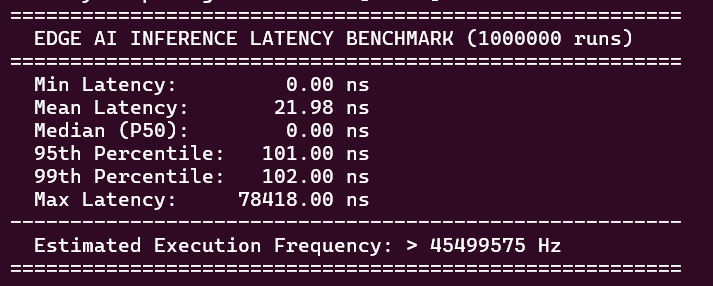
\includegraphics[width=0.62\linewidth]{figs/latency_benchmark.png}
\caption{Terminal output of the inference benchmark.}
\label{fig:latency}
\end{figure}
 
%==============================================================
\section{Discussion}\label{sec:discussion}
%==============================================================
\paragraph{Design rationale.} The central design choice is the separation of perception from control. The attitude loop runs on the IMU stream, whereas the perception workload runs on its own timer, and the two meet only through a boolean abort flag. This keeps the safety argument short: the gear can be deployed only if the interlock input is clear. The classifier is a short list of auditable comparisons rather than an opaque model.
 
\paragraph{What the results show.} In the static worlds the full chain from ranges to gear status behaves as intended, the slope estimate recovers the ramp inclination, and the classifier agrees with the world labels. These results demonstrate the data path and the interlock logic on idealised terrain.
 
\paragraph{Limitations.} The following limitations should be kept in mind.
\begin{itemize}
  \item \emph{Simulation fidelity.} The ToF sensors are noise-free, the terrains are rigid boxes and no optical penetration is modelled. Real ultrasonic transducers exhibit specular reflection from inclined surfaces, temperature-dependent speed of sound and cross-talk, and real ToF sensors are affected by ambient light and surface reflectivity. With realistic range noise, the short baselines of \cref{sec:geometry} amplify the noise to about $2^\circ$ per axis for 2\,mm.
  \item \emph{Data and score.} The dataset consists of three tight clusters recorded with an earlier sensing pipeline, the labels are assigned per world, and the thresholds are cluster midpoints. The perfect test score is therefore optimistic, and no evidence exists on unseen or mixed terrain. The tree was not retrained for the current feature definitions, which differ from the recorded columns.
  \item \emph{Class meaning.} On planar returns the second split acts as a second slope threshold, and the optical-acoustic features are not used, so the \textsc{unsafe\_vegetation} class is not shown to detect vegetation as such.
  \item \emph{Level-plate assumption.} The slope estimate uses neither the filtered attitude nor a surface normal, so body pitch and roll alias into slope, and the 0.1\,m patch scale limits what it can detect.
  \item \emph{No aerodynamic plant.} The airframe is held by a stand or carried on a rail, so the stabilator cannot change the body pitch. The pitch loop acts on the estimated pitch only, and the stability target of \cref{tab:accept} is not demonstrated.
  \item \emph{Supervisor.} The supervisor drives a prescribed trajectory, is not covered by the verification script, and has an ineffective pitch subscription (\cref{sec:supervisor}).
  \item \emph{Timing evidence.} The latency figure is a host measurement with a coarse clock. No embedded worst-case timing, task isolation or ARINC~653 compliance is claimed.
  \item \emph{Reduced hardware.} The bench prototype of \cref{sec:bench} uses one Uno, an IMU and a single ToF sensor, virtual actuators and provisional thresholds; it cannot estimate terrain slope or material, and its timing, accuracy and electrical behaviour were not characterised quantitatively.
\end{itemize}
 
\paragraph{Future work.} Natural extensions are (i) recording a new dataset with the current feature definitions, with noise, varied inclinations and mixed terrain, and a split by run or by geometry; (ii) a margin-based or debounced abort so that single noisy frames cannot toggle the interlock; (iii) compensation of the slope estimate with the filtered attitude, or a surface normal from the three points; (iv) a pitching-moment model so that the stabiliser loop is closed through the airframe; (v) enabling the prepared three-ToF configuration on the bench, with powered servos once the mechanics and the sign of the stabiliser command are checked; and (vi) porting the domains to the planned boards for hardware-in-the-loop tests.
 
%==============================================================
\section{Conclusion}\label{sec:conclusion}
%==============================================================
We presented a landing gear assistance system that judges whether the terrain below a descending UAV is suitable for landing and gates gear deployment accordingly. The simulation combines a three-domain architecture, a complementary-filter attitude estimator, an anti-windup PID pitch stabiliser, a slope estimate from the range differences of a triangular ToF array, a roughness measure and an optical-acoustic comparison, and a decision tree of two decision nodes that is compiled into allocation-free C++. A rate-limited gear controller ensures that an unsafe verdict dominates the deploy request. In three static worlds the verdict, abort flag and gear status were as expected, the measured ramp slope of 0.348\,rad matched the geometry, and the classifier scored 375 of 375 on a held-out split, a result explained by tight clusters and midpoint thresholds and not a measure of performance on real terrain. The host benchmark gave a mean inference time of 21.98\,ns with a clock resolution of about 100\,ns. A bench prototype on an Arduino Uno confirmed that attitude estimation, a virtual stabiliser command and rule-based readiness checks operate on real IMU and ToF data with the servos disconnected. Retraining on the current features, validation on noisy and mixed terrain, and hardware-in-the-loop tests are the next steps.
 
%==============================================================
\begin{thebibliography}{99}
\bibitem{repo} A.~Manitsas and M.~Vrana, \emph{LandingGearController: UAV Landing Gear Controller, Simulation and Hardware Prototype}, software repository (GPL-3.0), \url{https://github.com/AndrewManitsas/LandingGearController}.
\bibitem{arinc653} ARINC Specification 653, \emph{Avionics Application Software Standard Interface}, Aeronautical Radio, Inc.
\bibitem{ros2} S.~Macenski, T.~Foote, B.~Gerkey, C.~Lalancette and W.~Woodall, ``Robot Operating System 2: Design, architecture, and uses in the wild,'' \emph{Science Robotics}, vol.~7, no.~66, eabm6074, 2022.
\bibitem{gazebo} N.~Koenig and A.~Howard, ``Design and use paradigms for Gazebo, an open-source multi-robot simulator,'' in \emph{Proc.\ IEEE/RSJ Int.\ Conf.\ Intelligent Robots and Systems (IROS)}, 2004, pp.~2149-2154.
\bibitem{astrom} K.~J.~{\AA}str{\"o}m and R.~M.~Murray, \emph{Feedback Systems: An Introduction for Scientists and Engineers}, Princeton University Press, 2008.
\bibitem{cart} L.~Breiman, J.~H.~Friedman, R.~A.~Olshen and C.~J.~Stone, \emph{Classification and Regression Trees}, Wadsworth, 1984.
\bibitem{sklearn} F.~Pedregosa \emph{et al.}, ``Scikit-learn: Machine learning in Python,'' \emph{Journal of Machine Learning Research}, vol.~12, pp.~2825-2830, 2011.
\bibitem{vl53} STMicroelectronics, \emph{VL53L0X time-of-flight ranging sensor}, datasheet.
\bibitem{mpu6500} InvenSense, \emph{MPU-6500 Product Specification}.
\bibitem{fastimu} \emph{FastIMU}, Arduino library for inertial measurement units, distributed through the Arduino Library Manager.
\bibitem{pololu} Pololu Corporation, \emph{VL53L0X library for Arduino}, version 1.3.1.
\bibitem{hcsr04} \emph{HC-SR04 ultrasonic ranging module}, manufacturer datasheet.
\bibitem{mpu} InvenSense, \emph{MPU-9250 Product Specification}.
\bibitem{rp2350} Raspberry Pi Ltd, \emph{Raspberry Pi Pico 2 W and RP2350 datasheet}.
\bibitem{avr} Microchip Technology, \emph{ATmega328P datasheet}.
\bibitem{sg90} TowerPro, \emph{SG90 micro servo}, manufacturer datasheet.
\end{thebibliography}
 
\end{document}
 